\FloatBarrier
\section{Numerical Simulations} \label{sec:NumericalSims}
In order to evaluate the use of KIFMM in solving problems in stokes flow, we will look at Mobility problems where we can calculate the motion of swimmers in a stokes fluid.
\section{Mobility Problems}
The resistance problem is another common use of regularised stokes let where we obtain the rigid body motion prescribed force and moment. We can describe the motion of a single rigid body in a laboratory frame by defining  $\bm{\xi}$ to be the body frame of rigid body, then we can describe its position through the rotation matrix $B = [\bm{B}_1,\bm{B}_2,\bm{B}_3]$ where $B_i$ are basis vectors for the body frame and its origin point $\bm{x}_0$ relative to the laboratory frame. A position and velocity in the laboratory frame can be described by
\begin{equation*}
\begin{aligned}
    \bm{x} &= \bm{x}_0 + B\cdot\bm{\xi} \\
    \dot{\bm{x}} &= \dot{\bm{x}}_0 + \dot{B}\cdot\bm{\xi} + B\cdot\dot{\bm{\xi}}
\end{aligned}
\end{equation*}
We can redefine the velocity in terms of the rigid-body velocity $\bm{U}$ and angular velocity $\bm{\Omega}$ of the frame as
\begin{equation*}
    \dot{\bm{x}} = \bm{U} + \bm{\Omega}\times (\bm{x}-\bm{x}_0) + B\cdot\dot{\bm{\xi}}
\end{equation*}
The fluid flow can be described through the stokes flow equation defined in \cref{eq:BIE},
\begin{equation*}
    u_i(\bm{y}) = \frac{1}{8 \pi \mu} \int_{\partial D} S_{i j}^{\epsilon}\left(\bm{x}, \bm{y}\right) f_{j}(\bm{y}) d s(\bm{y}) \quad \forall \bm{x}\in\partial D
\end{equation*}
The nonslip boundary condition means that the velocity of the fluid on the boundary of the rigid body $\partial D$ is the same as the velocity of the boundary $\dot{\bm{x}}$
\begin{equation*}
    \bm{x}_i = \frac{1}{8 \pi \mu} \int_{\partial D} S_{i j}^{\epsilon}\left(\bm{x}, \bm{y}\right) f_{j}(\bm{y}) d s(\bm{y}) \quad \forall \bm{x}\in\partial D
\end{equation*}
By substituting the full equation for the velocity we can define the full Mobility problem as
\begin{equation}
\label{eq:MobilityProblem}
\begin{gathered}
    -U_{i}-\epsilon_{i j k} \Omega_{j}\left(x_{k}-x_{0 k}\right)+\frac{1}{8 \pi\mu} \iint_{\partial D} S_{i j}^{\epsilon}(\bm{x}, \bm{y}) f_{j}(\bm{y}) d S({\bm{y}})=B_{i j} \dot{\xi}_{j} \text { for all } \bm{x} \in \partial D, \\
    \iint_{\partial D} f_{i}(\bm{y}) d S({\bm{y}})=0 \\
    \iint_{\partial D} \epsilon_{i k j} y_{k} f_{j}(\bm{y}) d S({\bm{y}})=0,
\end{gathered}
\end{equation}
where $\epsilon_{ijk}$ is the Levi-Civita symbol. We have taken the total force and Moment on the body to be $0$ for the moment as we assume all external forces are negligible. Numerical discretisation of the problem leads to $3N$ scalar degrees of freedom in the traction $\bm{f}$ and a further $6$ scalar degrees of freedom to describe the total velocity $\bm{U}$ and angular momentum $\bm{\Omega}$ totalling $3N+6$ scalar degrees of freedom.

\subsection{Numerical Implementation}
The discretisation of the mobility problem is based on the same discretisation of that derived in \cref{sec:MRS} or though the use of the NEAREST (\cref{sec:NEAREST}) method. First condering the Nyström discretisation of Cortez et al \cite{Cortez2005} we replace the integrals in \cref{eq:MobilityProblem} with a numerical quadrature rule to obtain the problem.
\begin{equation*}
\begin{gathered}
    -U_{i}-\epsilon_{i j k} \Omega_{j}\left(x_k[{m}]-x_{0 k}\right)+\frac{1}{8 \pi\mu} \sum_{n=1}^N S_{i j}^{\epsilon}(\bm{x}_m, \bm{x}_n) f_{j}(\bm{x}_n) A_n =  B_{i j} \dot{\xi}_{j}[m] \\ \text { for all } m = 1,\dots,N\\
    \sum_{n=1}^N f_{i}(\bm{x}_n) A_n=0 \\
    \sum_{n=1}^N \epsilon_{i k j} x_{k}[n] f_{j}(\bm{x}_n) A_n=0,
\end{gathered}
\end{equation*}
where $x_{i}[n]$ denotes the the position of the $n$th quadrature point in the $i$th axis and $A_n$ the qudarture weight at the point $\bm{x}_n$. We have again considered the Nyström discretisation for this problem to aid such that we have a well defined problem for which we can compute the solution to the linear system. Through the use of the a nearest neighbour matrix (\cref{eq:NNMatrix})
\begin{equation*}
    \nu [q, \hat{n}]= \begin{cases} 1/k & \text { if } \hat{n}=\underset{n=1, \ldots, N}{\operatorname{argmin}}|x_n-X_q| , \\ 0 & \text { otherwise. }\end{cases}
\end{equation*}
where $k$ is the number of points in $\{x_n\}$ which are equidistant to $\{X_q\}$ we can perform the same discretisation seen in \cref{sec:NEAREST} to obtain.
\begin{equation*}
\begin{gathered}
    -U_{i}-\epsilon_{i j k} \Omega_{j}\left(x_k[{m}]-x_{0 k}\right)+\frac{1}{8 \pi\mu} \sum_{n=1}^N f_{j}(\bm{x}_n) A_n \sum_{q=1}^Q S_{i j}^{\epsilon}(\bm{x}_m, \bm{X}_q)\nu [q, n]  =  B_{i j} \dot{\xi}_{j}[m] \\ \text { for all } m = 1,\dots,N\\
    \sum_{n=1}^N f_{i}(\bm{x}_n) A_n \sum_{q=1}^Q \delta_{i j}\nu [q, n]= 0 \\
    \sum_{n=1}^N f_{j}(\bm{x}_n) A_n \sum_{q=1}^Q \epsilon_{i k j} X_{k}[q] \nu [q, n] = 0,
\end{gathered}
\end{equation*}
Both discretisation correspond to $3N + 6$ equations in $3N + 6$ unknowns $F_j(\bm{x}_n)$, $U_j$ and $\Omega_j$ for $n=1,\dots,N$ and $j=1,2,3$. We can consider this equation in terms of a block matrix form as we did for the resistance problem (\cref{sec:resistance}) where we augment the force vector of unknowns with the velocity $\boldsymbol{U}$ and angular velocity $\boldsymbol{\Omega}$ which are both $3 \times 1$ column vectors. The right hand side of the equation is augmented with two $3 \times 1$ column vectors of zeros which denote the prescribed zero total force and moment on the rigid body. This gives us a final form of our block matrix system as
\begin{equation}
\label{eq:mobilityStructure}
\arraycolsep=0.4pt\def\arraystretch{1}
\left(
\begin{array}{cc}
\begin{array}{ccc}
A_{11} & A_{12} & A_{13} \\
A_{21} & A_{22} & A_{23} \\
A_{31} & A_{32} & A_{33}
\end{array} &
\begin{array}{cc}
B_{1}^{U} & B_{1}^{\Omega} \\
B_{2}^{U} & B_{2}^{\Omega} \\
B_{3}^{U} & B_{3}^{\Omega} \\
\end{array} \\
\begin{array}{ccc}
B_{1}^{F} & B_{2}^{F} & B_{3}^{F} \\
B_{1}^{M} & B_{2}^{M} & B_{3}^{M}
\end{array} & \bm{0}_{6 \times 6}
\end{array}
\right)
\left(\begin{array}{c}
F_{1}({\bm{x}}_{1}) \\
\vdots \\
F_{1}({\bm{x}}_{N}) \\
F_{2}({\bm{x}}_{1}) \\
\vdots \\
F_{2}({\bm{x}}_{N}) \\
F_{3}({\bm{x}}_{1}) \\
\vdots \\
F_{3}({\bm{x}}_{N}) \\
\boldsymbol{U} \\
\boldsymbol{\Omega}
\end{array}\right)=\left(\begin{array}{c}
B_{1 j} \dot{\xi}_{j}({\bm{x}}_{1}) \\
\vdots \\
B_{1 j} \dot{\xi}_{j}({\bm{x}}_{N}) \\
B_{2 j} \dot{\xi}_{j}({\bm{x}}_{1}) \\
\vdots \\
B_{2 j} \dot{\xi}_{j}({\bm{x}}_{N}) \\
B_{3 j} \dot{\xi}_{j}({\bm{x}}_{1}) \\
\vdots \\
B_{3 j}\dot{\xi}_{j}({\bm{x}}_{N}) \\
\mathbf{0}_{3 \times 1} \\
\mathbf{0}_{3 \times 1}
\end{array}\right),
\end{equation}
where the blocks for the Nyström discretisation are given as
\begin{equation*}
\begin{aligned}
A_{ij}(m,n) &= \frac{1}{8\pi\mu} S_{ij}^\epsilon (\bm{x}_m,\bm{x}_{n}) \text { for } m,n = 1,\dots,N \\
B_{i}^{U}(m,j) &= -\delta_{ij} \text { for } m = 1,\dots,N \\
B_{i}^{\Omega}(m,j) &= -\epsilon_{ijk}(x_k[m]-x_{0k}) \text { for } m = 1,\dots,N \\
B_{j}^{F}(i,n) &= \delta_{ij} \text { for } n = 1,\dots,N \\
B_{j}^{M}(i,n) &= \epsilon_{ikj} x_k[n] \text { for } n = 1,\dots,N
\end{aligned}
\end{equation*}
or for the NEAREST discretisation
\begin{equation*}
\begin{aligned}
A_{ij}(m,n) &= \frac{1}{8\pi\mu} \sum_{q=1}^Q S_{ij}^\epsilon (\bm{x}_m,\bm{X}_{q})\nu[q,n] \text { for } m,n = 1,\dots,N \\
B_{i}^{U}(m,j) &= -\delta_{ij} \text { for } m = 1,\dots,N \\
B_{i}^{\Omega}(m,j) &= -\epsilon_{ijk}(x_k[m]-x_{0k}) \text { for } m = 1,\dots,N \\
B_{j}^{F}(i,n) &= \delta_{ij} \sum_{q=1}^Q \nu[q,n] \text { for } n = 1,\dots,N \\
B_{j}^{M}(i,n) &= \epsilon_{ikj} \sum_{q=1}^Q X_k[q] \nu[q,n] \text { for } n = 1,\dots,N
\end{aligned}
\end{equation*}

\subsection{Boundaries}
Often when working with stokes flow we wish to include boundaries in our numerical simulation. These might be simulating microswimmers sandwiched between a microscope slides and a coverslip \cite{Gallagher2019RapidAnalysis} or simulating blood cells in cylindrical arteries, any such boundary will have a noticeable effect on the stokeslets and therefore the rigid body motion \cite{Liron1981ExistenceBoundaries}. While solutions around large infinite planes can be simulated through the use of the Blakelet solution \cite{Ainley2008TheStokeslets,Cortez2015}, more complex geometry requires the use of a quadrature rule of over the boundary $B$. Taking the boundary of $B$ to be $\partial B$
\begin{equation}
\label{eq:MobilityProblemBnd}
\begin{gathered}
    -U_{i}-\epsilon_{i j k} \Omega_{j}\left(x_{k}-x_{0 k}\right)+\frac{1}{8 \pi\mu} \iint_{\partial D \cup \partial B} S_{i j}^{\epsilon}(\bm{x}, \bm{y}) f_{j}(\bm{y}) d S({\bm{y}})=B_{i j} \dot{\xi}_{j} \text { for all } \bm{x} \in \partial D, \\
    \iint_{\partial D \cup \partial B} S_{i j}^{\epsilon}(\bm{x}, \bm{y}) f_{j}(\bm{y}) d S({\bm{y}}) = \dot{x}_i \text { for all } \bm{x} \in \partial B \\
    \iint_{\partial D} f_{i}(\bm{y}) d S({\bm{y}})=0 \\
    \iint_{\partial D} \epsilon_{i k j} y_{k} f_{j}(\bm{y}) d S({\bm{y}})=0,
\end{gathered}
\end{equation}
This addition to the problem is numerically solved in the same way as for the single swimmer, by introducing a second discretisation (or third and fourth discretisation in the case of NEAREST) of the boundary $\partial B$. Now taking the original number of quadrature points to be $N_D$ and the set of new quadrature points $\{\bm{x}_n\}$ where $n=N_D+1,\dots,N_B$. Discretisation of the problem leads to the same block structure described in \cref{eq:mobilityStructure} however with different block components in order to compute the new boundary conditions. For the single quadrature rule discetisation we obtain the block structure
\begin{equation*}
\begin{aligned}
A_{ij}(m,n) &= \frac{1}{8\pi\mu} S_{ij}^\epsilon (\bm{x}_m,\bm{x}_{n}) \text { for } m,n = 1,\dots,N_s,N_D+1,\dots,N_D+N_B \\
B_{i}^{U}(m,j) &= \begin{cases} -\delta_{ij} \text { for } m = 1,\dots,N_D \\ 0 \text { for } m = N_D+1,\dots,N_D+N_B\end{cases} \\
B_{i}^{\Omega}(m,j) &= \begin{cases} -\epsilon_{ijk}(x_k[m]-x_{0k}) \text { for } m = 1,\dots,N \\ 0 \text { for } m = N_D+1,\dots,N_D+N_B\end{cases} \\
B_{j}^{F}(i,n) &= \begin{cases} \delta_{ij} \text { for } n = 1,\dots,N \\ 0 \text { for } n = N_D+1,\dots,N_D+N_B\end{cases} \\
B_{j}^{M}(i,n) &= \begin{cases} \epsilon_{ikj} x_k[n] \text { for } n = 1,\dots,N \\ 0 \text { for } n = N_D+1,\dots,N_D+N_B\end{cases}
\end{aligned}
\end{equation*}
and for the NEAREST discretisation where the coarse force discretisation is extended in the same way as the Nyström discretisation $\{\bm{x}_n\}$ where $n=1,\dots,N_D+N_B$ and a fine quadrature rule $\{\bm{X}_q\}$ where $q=1,\dots,Q=Q_D+Q_B$
\begin{equation*}
\begin{aligned}
A_{ij}(m,n) &= \frac{1}{8\pi\mu} \sum_{q=1}^Q S_{ij}^\epsilon (\bm{x}_m,\bm{X}_{q})\nu[q,n] \text { for } m,n = 1,\dots,N_s,N_D+1,\dots,N_D+N_B  \\
B_{i}^{U}(m,j) &= \begin{cases} -\delta_{ij} \text { for } m = 1,\dots,N \\ \text { for } m = N_D+1,\dots,N_D+N_B\end{cases}\\
B_{i}^{\Omega}(m,j) &= \begin{cases} -\epsilon_{ijk}(x_k[m]-x_{0k}) \text { for } m = 1,\dots,N \\ \text { for } m = N_D+1,\dots,N_D+N_B\end{cases}\\
B_{j}^{F}(i,n) &= \begin{cases} \delta_{ij} \sum_{q=1}^Q \nu[q,n] \text { for } n = 1,\dots,N \\ 0 \text { for } n = N_D+1,\dots,N_D+N_B\end{cases} \\
B_{j}^{M}(i,n) &= \begin{cases} \epsilon_{ikj} \sum_{q=1}^Q X_k[q] \nu[q,n] \text { for } n = 1,\dots,N \\ 0 \text { for } n = N_D+1,\dots,N_D+N_B\end{cases}.
\end{aligned}
\end{equation*}
This is now as system of $3N = 3N_D+3N_B + 6$ unknowns in $3N$ equations. The Vector of unknowns is again arranged as in \cref{eq:mobilityStructure} where $N=N_D+N_B$. Writing the right hand side as $(V_1,V_2,V_3)^T$ we can write that
\begin{equation*}
    V_i[n] = \begin{cases} B_{i j} \dot{\xi}_{j}({\bm{x}}_{n}) \text{ for } n=1,\dots,N_D \\ \dot{x}_i[n] \text{ for } n=N_D+1,\dots,N_D+N_B \end{cases}
\end{equation*}

\section{Multiple Swimmers}
It is often the cases that systems will contain multiple rigid bodies of either the same type or different types. If we consider $N_{sw}$ swimmers then we can write for the case of the mobility problem with boundaries that
\begin{equation}
\label{eq:MobilityProblemMulti}
\begin{gathered}
    -U_{i}[n]-\epsilon_{i j k} \Omega_{j}[n]\left(x_{k}[n]-x_{0 k}[n]\right)+\frac{1}{8 \pi\mu} \iint_{\partial D \cup \partial B} S_{i j}^{\epsilon}(\bm{x}, \bm{y}) f_{j}(\bm{y}) d S({\bm{y}})=B_{i j}[n] \dot{\xi}_{j}[n] \\ \text { for all } \bm{x} \in \partial D[n], \\
    \iint_{\partial D \cup \partial B} S_{i j}^{\epsilon}(\bm{x}, \bm{y}) f_{j}(\bm{y}) d S({\bm{y}}) = \dot{x}_i \text { for all } \bm{x} \in \partial B \\
    \iint_{\partial D[n]} f_{i}(\bm{y}) d S({\bm{y}})=0 \\
    \iint_{\partial D[n]} \epsilon_{i k j} y_{k} f_{j}(\bm{y}) d S({\bm{y}})=0,
\end{gathered}
\end{equation}
for each $n=1,\dots,N_{sw}$ where $\partial D[n]$ is the boundary of the $n$th swimmer and $\partial D = \bigcup_{n=1}^{N_{sw}} \partial D[n]$. The numerical discretisation of \cref{eq:MobilityProblemMulti} is similar to that of  \cref{eq:MobilityProblem} or \cref{eq:MobilityProblemBnd} and retains the same block structure as \cref{eq:mobilityStructure} , however is significantly more notionally complex, partially when the number of points discretising each swimmer is different. For this reason we will only consider the more complex NEAREST discretisation where the Nyström can be obtained in the limiting case where the coarse force discritisation and fine quadrature rule are identical and $\nu = I_{N \times N}$.

If we consider the $N_{sw}$ swimmers to have collocation points $x_i^{(1)}[\cdot],\dots,x_i^{(N_{sw})}[\cdot]$ where $x_i^{(1)}[\cdot]$ denotes all the $i$th components of the first swimmers collocation points and $x_i^{(B)}[\cdot]$ is the $i$th components of the boundaries collocation points. Using the same ordering convention used in the previous section we have that
\begin{equation*}
    \bm{x} = (\bm{x}_1,\bm{x}_2,\bm{x}_3)^T \text{ with } \bm{x}_1=(x_i^{(1)}[\cdot],\dots,x_i^{(N_{sw})}[\cdot],x_i^{(B)}[\cdot])
\end{equation*}
The translational and angualar velocities are given by $U_i^{(1)},\dots,U_i^{(N_{sw})}$ and $\Omega_i^{(1)},\dots,\Omega_i^{(N_{sw})}$ respectively and the the boundary collocation points by $x_i^{(b)}[\cdot]$. The ordering of discritisation remains the same as \cref{eq:mobilityStructure} where if we denote the vector of unknowns as $(\bm{F}_1, \bm{F}_2, \bm{F}_3, \bm{U}_1,\bm{U}_2,\bm{U}_3,\bm{\Omega}_1,\bm{\Omega}_2,\bm{\Omega}_3)^T$ where $\bm{F}_i = (F_i^{(1)}[\cdot],\dots,F_i^{(N_{sw})}[\cdot],F_i^{(b)}[\cdot])$, $\bm{U}_i = (U_i^{(1)},\dots,U_i^{(N_{sw})})^T$ and $\bm{\Omega}_i = (\Omega_i^{(1)},\dots,\Omega_i^{(N_{sw})})^T$. The same ordering convention is used for the right hand side velocities, total forces and moments. If the number of force points associated with a swimmer $s$ is $N_{D}(s)$ and the number of force points on the boundary is $N_B$ then the total number of points is $N_F=\sum_{s=1}^{N_{sw}} N_D(s) + N_B$. We will also define an index $\iota(s)=\sum_{\alpha=1}^{s-1}N_D(\alpha)$ for $1<s\leq N_{sw}$ to be the location of the $s$th swimmer in $\bm{x}_i$, as $\iota(s)$ is defined above for all of $1<s\leq N_{sw}$ we also define $\iota(1)=1$. The ordering of the fine quadrature points is arbitrary due to its mapping through $\nu$, we will denote this set as $\{\bm{X}_q\}$ for $q=1,\dots{Q}$ as we have before. The Stokeslet matrix remains the same and is constructed by
\begin{equation*}
    A_{ij}(\alpha,\beta) = \frac{1}{8\pi\mu} \sum_{q=1}^Q S_{ij}^\epsilon (\bm{x}_\alpha,\bm{X}_{q})\nu[q,\beta] \text { for } \alpha,\beta = 1,\dots,N_F
\end{equation*}
Defining $\bm{1}^{(n)}$ to be a column vector of ones with length $n$ and $\bm{0}^{(m\times n)}$ to be a $(m\times n)$ matrix of zeros. We can therefore define the $N_F \times N_{sw}$ matrices
\begin{equation*}
\arraycolsep=0.4pt\def\arraystretch{1}
    \tilde{x}_i(\cdot,\cdot)=\left(\begin{array}{c}
         \begin{array}{ccc}
             x_i^{(1)}[\cdot]-x_{0i}^{(1)} & & \\
              & \ddots & \\
              & & x_i^{(N_{sw})}[\cdot]-x_{0i}^{(N_{sw})}
         \end{array}\\
         \bm{0}^{(N_B \times N_{sw})}
    \end{array}\right).
\end{equation*}
Then
\begin{equation*}
\arraycolsep=0.4pt\def\arraystretch{1}
    B^U = \mathds{1}_{3} \otimes \left(\begin{array}{c}
         \begin{array}{ccc}
             -\bm{1}^{(N_D(1))} & & \\
              & \ddots & \\
              & & -\bm{1}^{(N_D(N_{sw}))}
         \end{array}\\
         \bm{0}^{(N_B \times N_{sw})}
    \end{array}\right), \;
    B^\Omega =
    \left(\begin{array}{ccc}
             & -\tilde{x}_3(\cdot,\cdot) & \tilde{x}_2(\cdot,\cdot)\\
            \tilde{x}_3(\cdot,\cdot) & & -\tilde{x}_1(\cdot,\cdot)\\
            -\tilde{x}_2(\cdot,\cdot) & \tilde{x}_1(\cdot,\cdot) &
          \end{array}\right)
\end{equation*}
with $\mathds{1}_{3}$ denoting the $3\times3$ identity matrix and $\otimes$ the Kronecker product.
In order to construct the $N_{sw} \times N_F$ matrices we define two $1 \times N_D(s)$ row vectors
\begin{equation*}
\begin{aligned}
    \lambda^{(s)}[\cdot] &= \sum_{q=1}^Q \nu[q,\gamma] \text{ for } \gamma = \iota(s),\cdots,\iota(s+1)-1 \text{ and } \\
    \chi_j^{(s)}[\cdot] &= \sum_{q=1}^{Q} X_j(q)\nu[q,\gamma] \text{ for } \gamma = \iota(s),\cdots,\iota(s+1)-1
\end{aligned}
\end{equation*}
these allow us to define
\begin{equation*}
\arraycolsep=0.4pt\def\arraystretch{1}
    \tilde{\chi}_j(\cdot,\cdot)=\left(\begin{array}{cc}
         \begin{array}{ccc}
             \chi_j^{(1)}[\cdot] & & \\
              & \ddots & \\
              & & \chi_j^{(N_{sw})}[\cdot]
         \end{array} & \bm{0}^{(N_{sw} \times N_B)}
    \end{array}\right).
\end{equation*}
Then
\begin{equation*}
\arraycolsep=0.4pt\def\arraystretch{1}
    B^F = \mathds{1}_{3} \otimes \left(\begin{array}{cc}
         \begin{array}{ccc}
             \lambda^{(1)}[\cdot] & & \\
              & \ddots & \\
              & & \lambda^{(N_{sw})}[\cdot]
         \end{array} & \bm{0}^{(N_{sw} \times N_B)}
    \end{array}\right), \;
    B^M =
    \left(\begin{array}{ccc}
             & -\tilde{\chi}_3(\cdot,\cdot) & \tilde{\chi}_2(\cdot,\cdot)\\
            \tilde{\chi}_3(\cdot,\cdot) & & -\tilde{\chi}_1(\cdot,\cdot)\\
            -\tilde{\chi}_2(\cdot,\cdot) & \tilde{\chi}_1(\cdot,\cdot) &
          \end{array}\right)
\end{equation*}
Finally defining the right hand side vector as $(\bm{V}_1,\bm{V}_1,\bm{V}_1,\bm{0}_{(6N_{sw} \times 1)})^T$ where
\begin{equation*}
    V_i^{(s)} = (B_{ij}^{(1)}\dot{\xi}_j^{(1)}[\cdot],\dots,B_{ij}^{(N_{sw})}\dot{\xi}_j^{(N_{sw})}[\cdot],\dot{x}_i[1],\dots,\dot{x}_i[N_B])
\end{equation*}
This allows us to form the full system of $3(N_F+2N_{sw})\times3(N_F+2N_{sw})$ system of linear equations e given in the same structure as \cref{eq:mobilityStructure}.

We will be solving this system through the use of GMRES (see \cref{appendix:GMRES}) as we are unable to form the full matrix with the KIFMM method. We can instead compute the matrix in block, we will compute the stokeslet matrix $A$ with the KIFMM method first before constructing the $B_i^U$, $B_i^\Omega$, $B_i^F$ and $B_i^M$ matrix blocks. For notational ease we will group these into two matrices
\begin{equation*}
B = \left( \begin{array}{ccc}
B_{1}^{F} & B_{2}^{F} & B_{3}^{F} \\
B_{1}^{M} & B_{2}^{M} & B_{3}^{M}
\end{array}\right) \text{ and }
B^T = \left(\begin{array}{cc}
B_{1}^{U} & B_{1}^{\Omega} \\
B_{2}^{U} & B_{2}^{\Omega} \\
B_{3}^{U} & B_{3}^{\Omega} \\
\end{array}\right).
\end{equation*}





\subsection{Rods in Shear flow}
In order to benchmark the use of KIFMM in the case of swimming problems, we propose to look at the problem of rods in a shear flow. We will consider prolate spheroid rods with a minor axis of $0.15$ and a major axis of $1$ arranged in a triangular lattice with a rod to rod spacing of $0.4$. In order to impose motion on the rods, a shear flow is imposed on the fluid such that the rods want to locally rotate about the $x_2$ axis. This is imposed by setting the fluid velocity of each force point on the swimming problem to be $\bm{u} = (\gamma\cdot x_3,0,0)$ where $\gamma$ denotes the magnitude of the shear flow and $x_3$ the z coordinate of the force points positions. We consider the two versions of the problem, each having approximately the same number of quadrature points but with a varying number of swimmers. The first problem involves 203 rods arranged in a triangular lattice of size $[5.2 \times 5.2]$ each is discretised with 420 quadrature points for a total of 255780 scalar degrees of freedom (SDOF). The second problem is 2016 rods discretised with 42 quadrature points for a total of 254,016 SDOF.  For the KIFMM method, we will use 500 particles in a node with 152 quadrature points as this provides an acceptably accurate approximation to the vector product while still keeping computation times reasonable. A regularisation parameter of $\epsilon=10^{-2}$ was set to allow for regularisation error and a standard Nyström was implemented such that the performance of just the KIFMM method for swimming problems was being assessed. The use of NEAREST implementation can be considered later in the case of Squirmers. Due to the complexity of the fluid system with a large number of degrees of freedom and close boundaries we will also consider optimisation to the method which could help reduce the overall computation time of the problem in the hope of allowing for larger-scale problems to be considered in the future. 


\begin{figure}[!ht]
        \centering
        \begin{subfigure}[b]{0.475\textwidth}
            \centering
            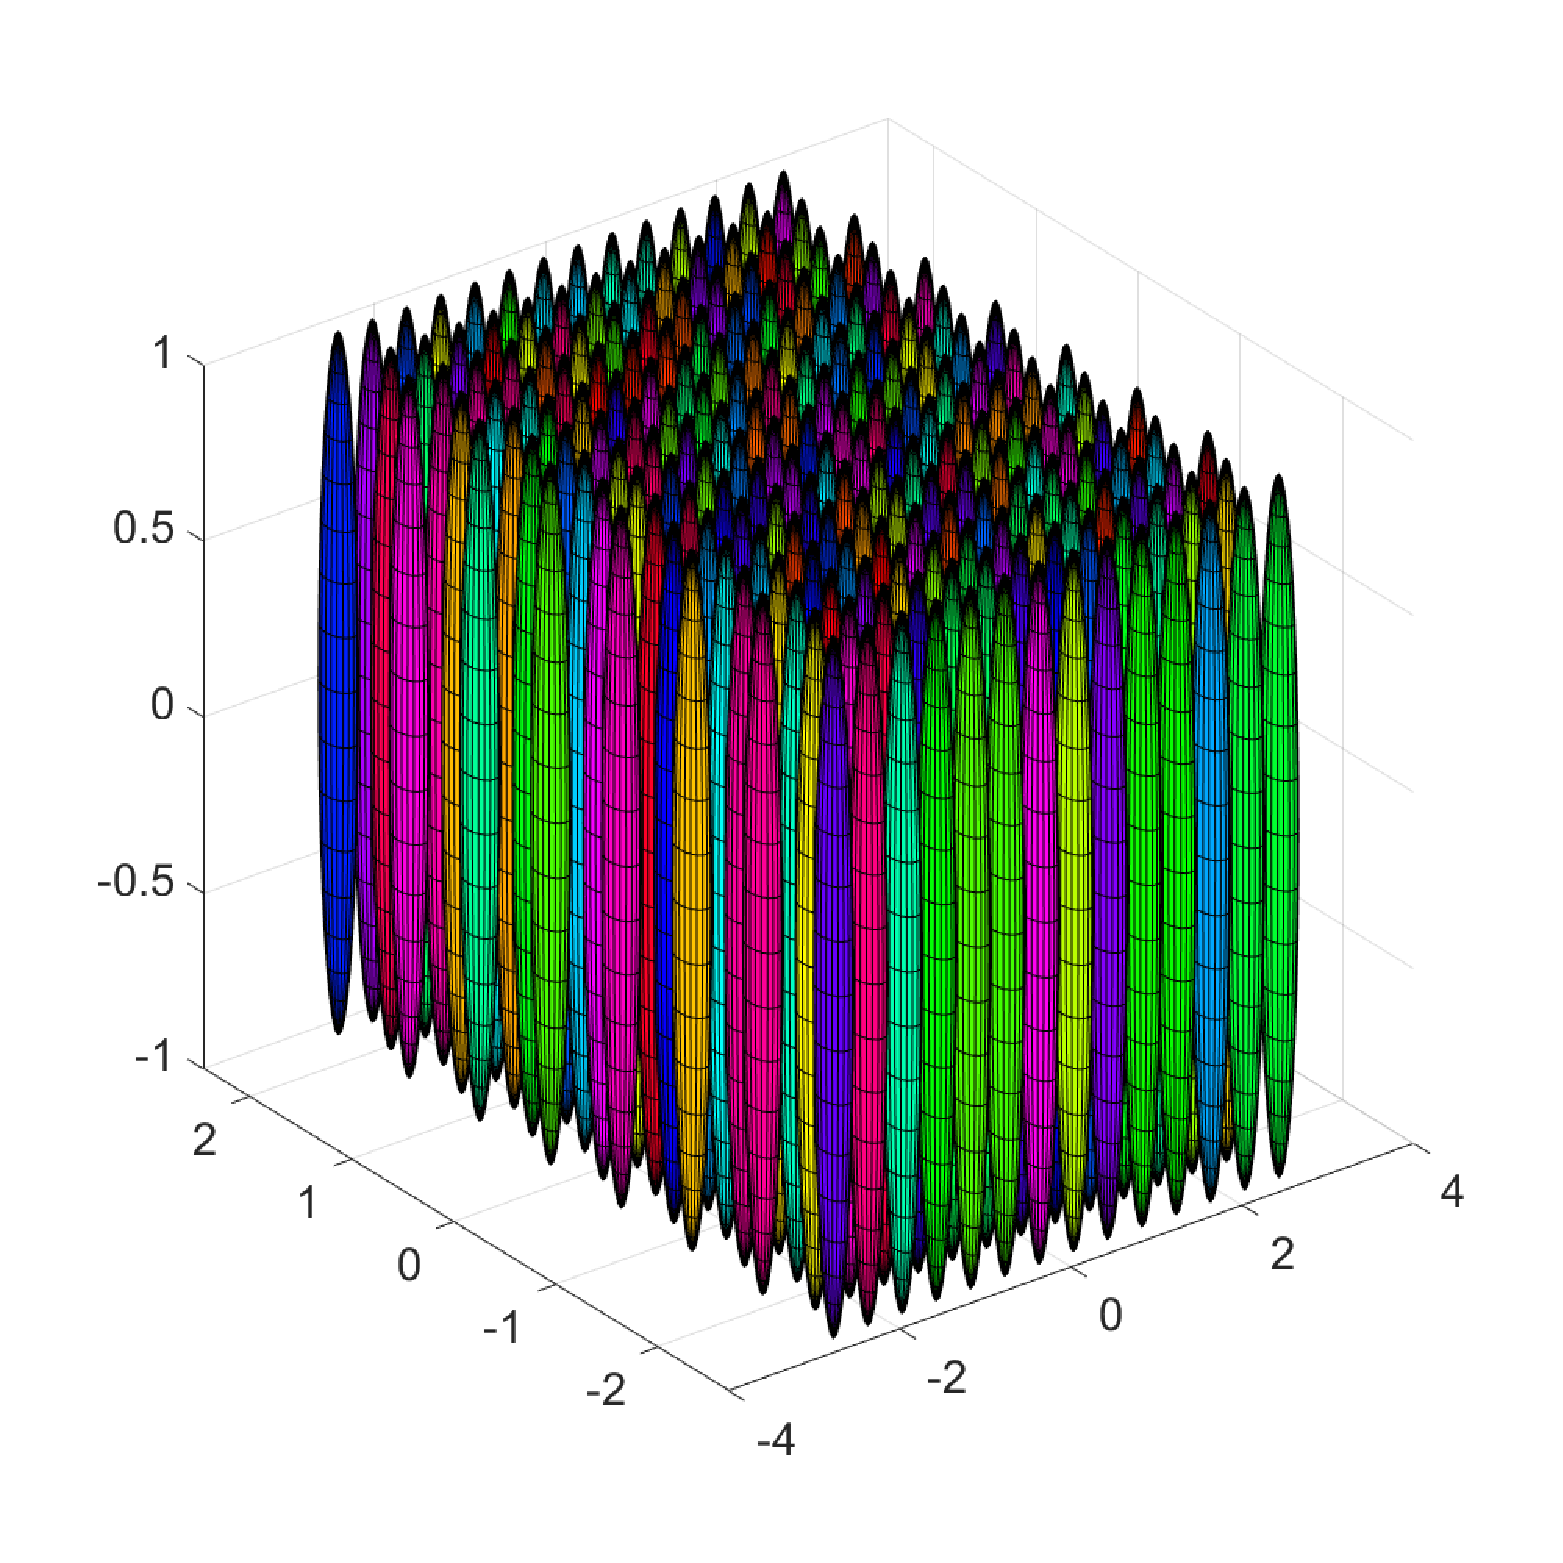
\includegraphics[width=\textwidth]{Images/Rods/SmallRods3d.pdf}
            \caption[]%
            {{\small 203 prolate spheroids in 3d View}}    
            \label{fig:mean and std of net14}
        \end{subfigure}
        \begin{subfigure}[b]{0.475\textwidth}  
            \centering 
            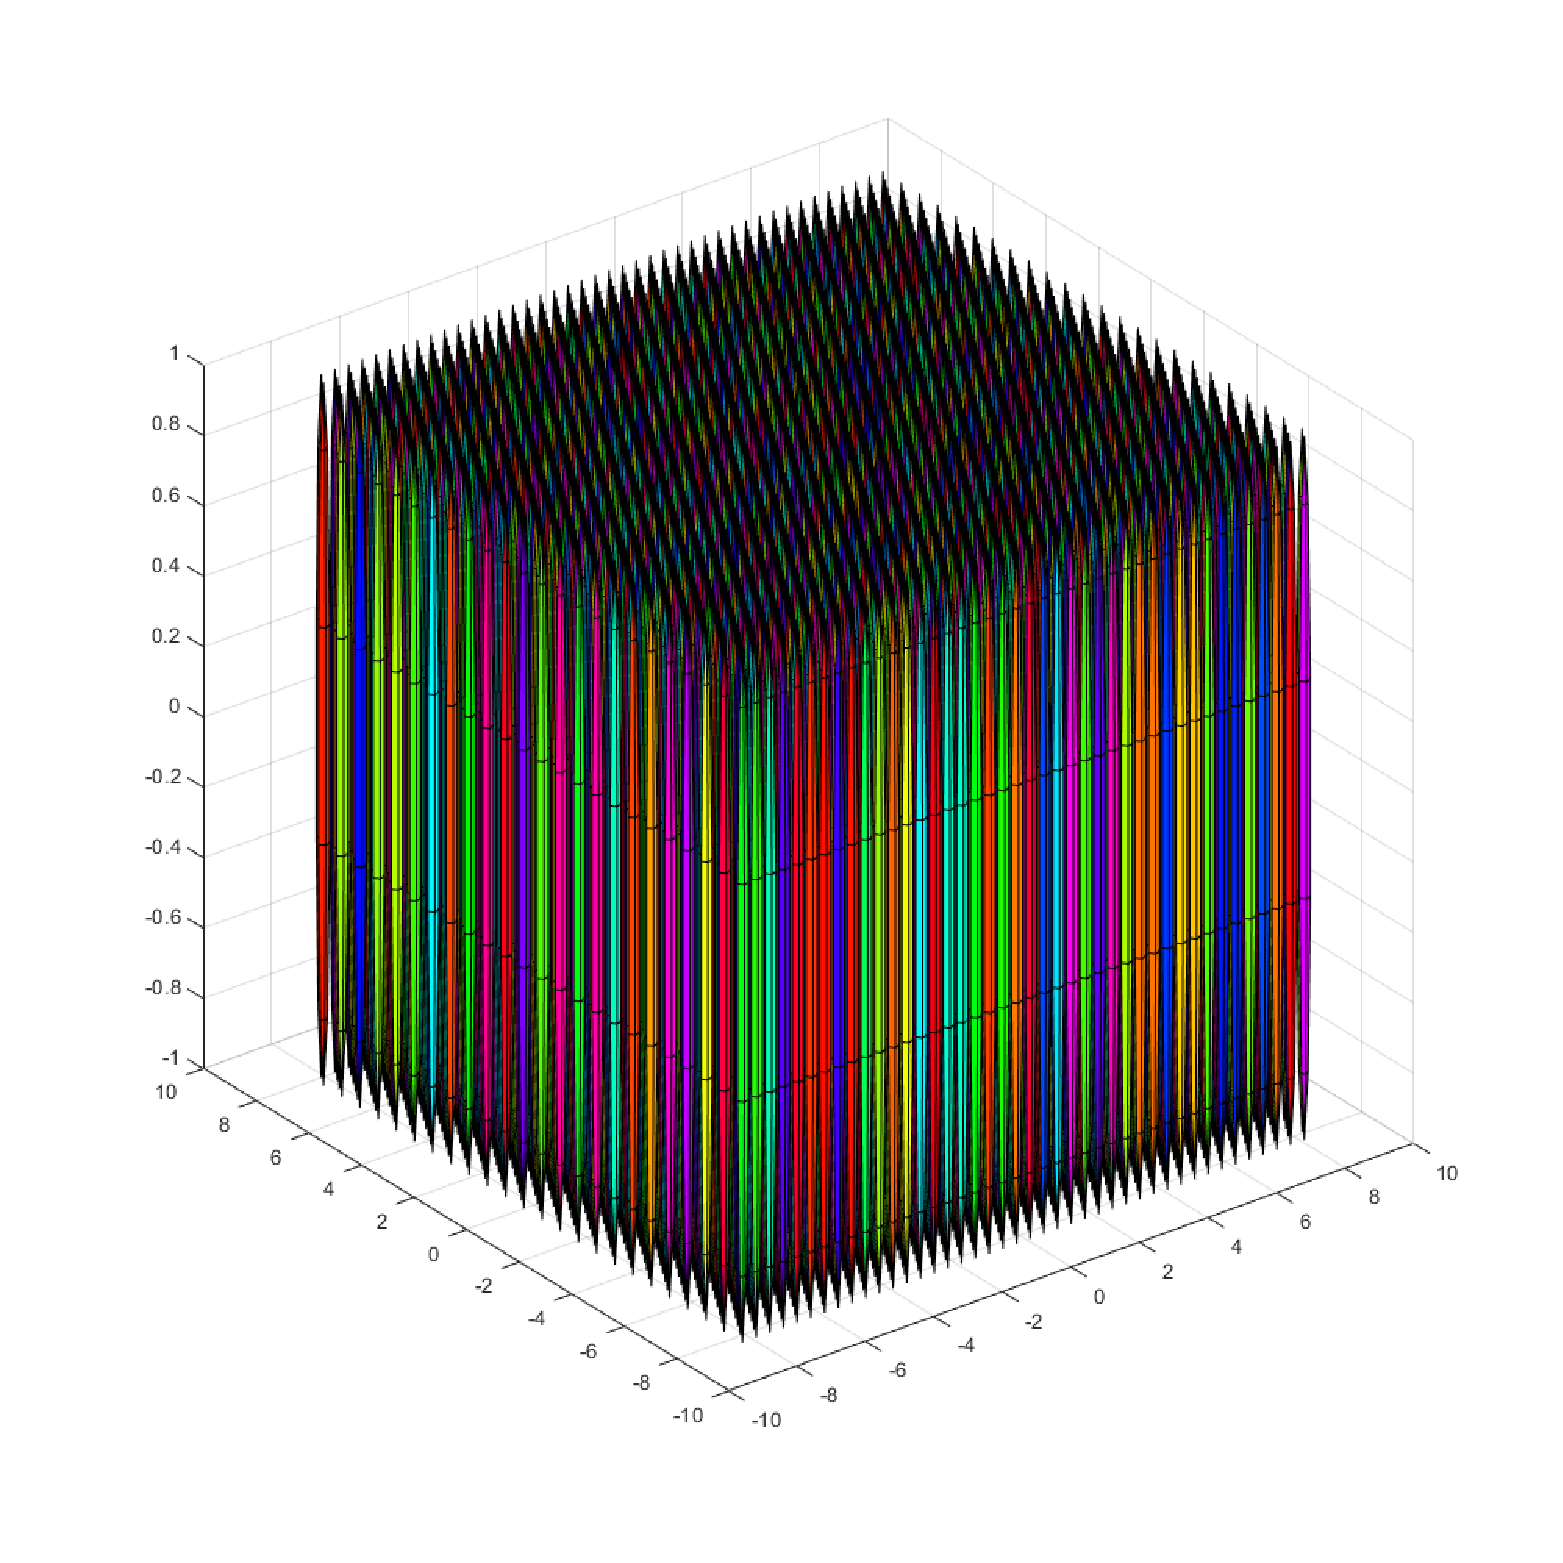
\includegraphics[width=\textwidth]{Images/Rods/LargeRods3d.pdf}
            \caption[]%
            {{\small 2016 prolate spheroids in 3d View}}    
            \label{fig:mean and std of net24}
        \end{subfigure}
        \vskip\baselineskip
        \begin{subfigure}[b]{0.475\textwidth}   
            \centering 
            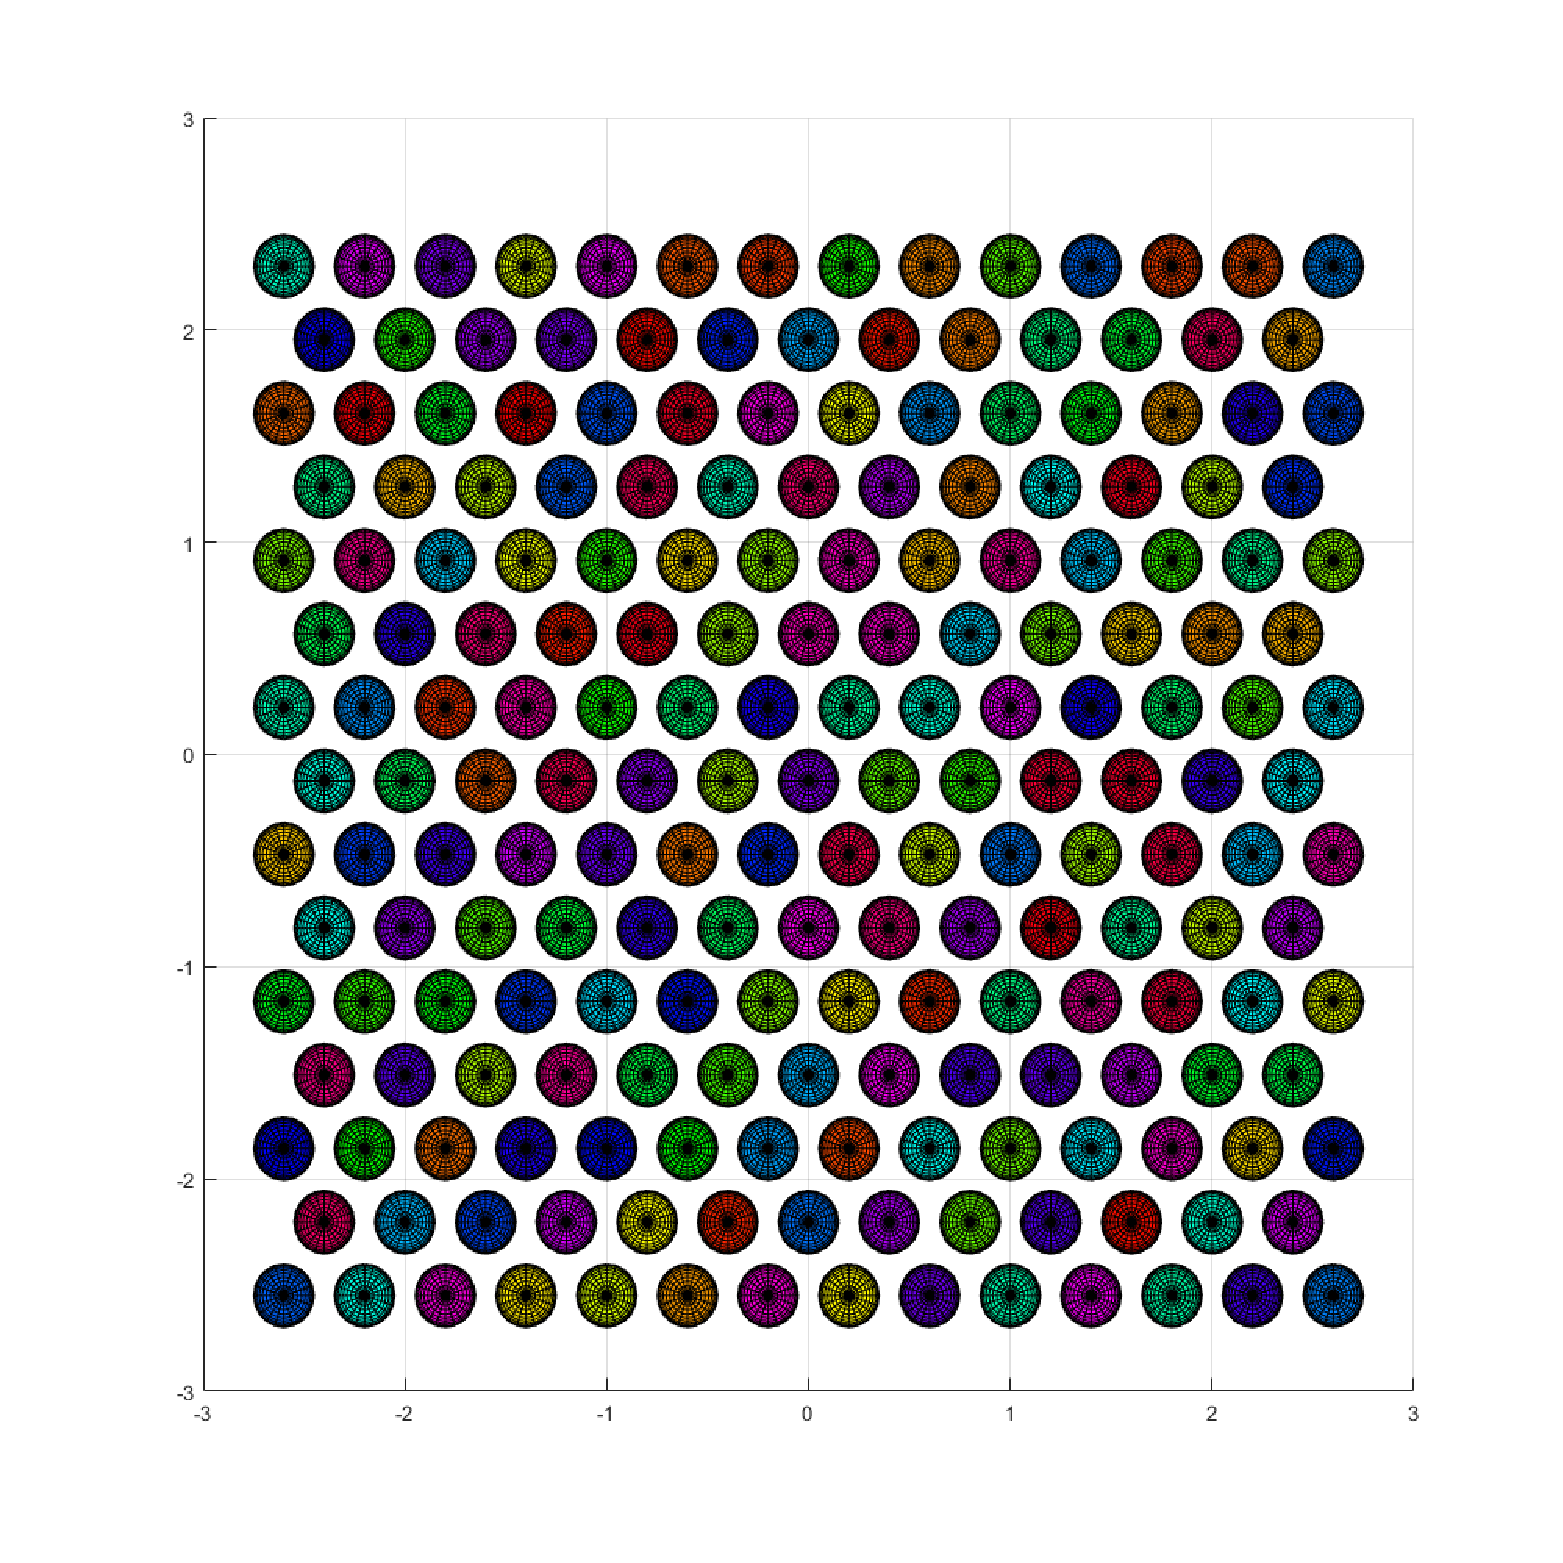
\includegraphics[width=\textwidth]{Images/Rods/SmallRodstop.pdf}
            \caption[]%
            {{\small 203 prolate spheroids from top down view}}    
            \label{fig:mean and std of net34}
        \end{subfigure}
        \hfill
        \begin{subfigure}[b]{0.475\textwidth}   
            \centering 
            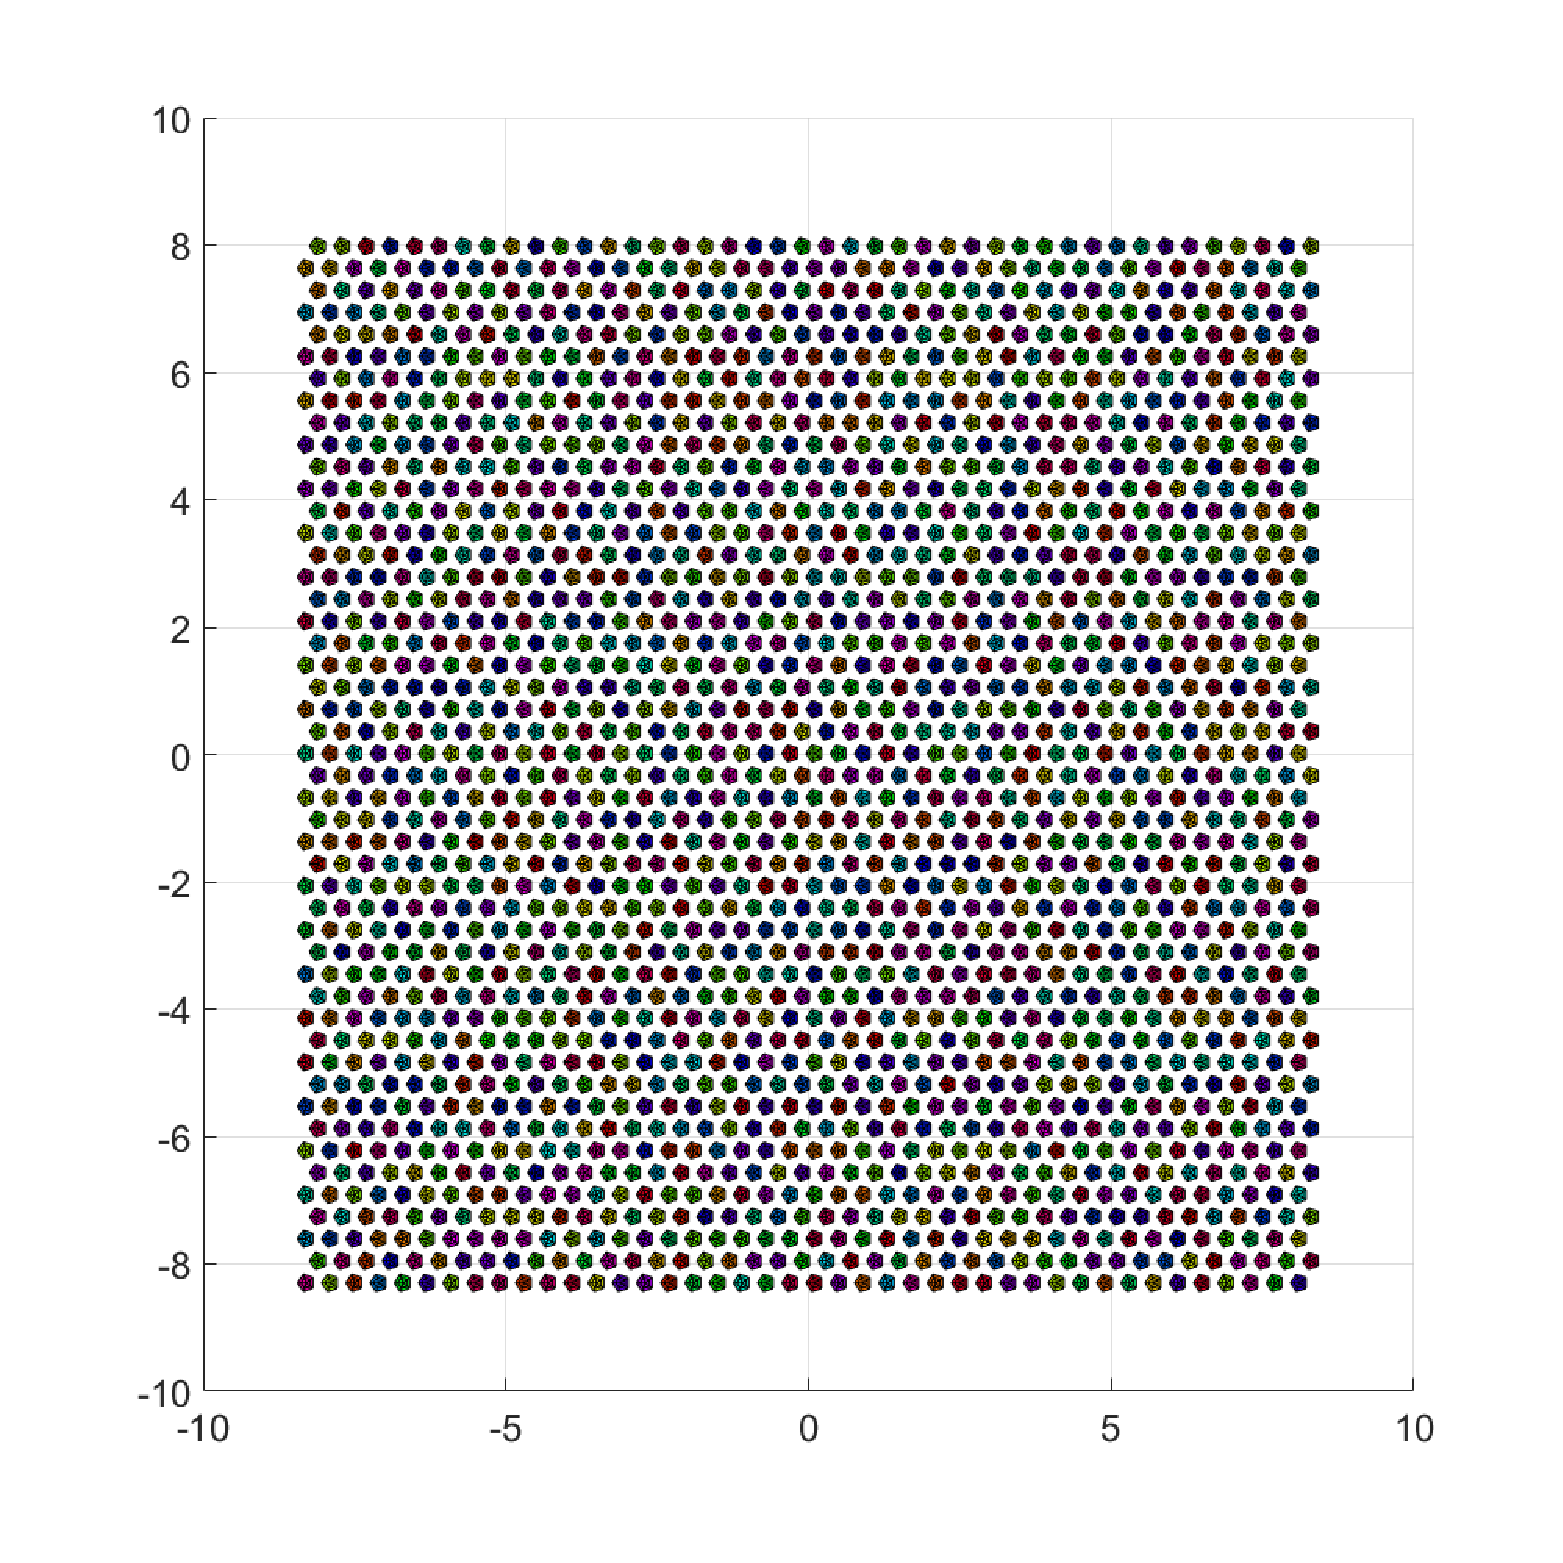
\includegraphics[width=\textwidth]{Images/Rods/LargeRodstop.pdf}
            \caption[]%
            {{\small 2016 prolate spheroids from top down view}}    
            \label{fig:mean and std of net44}
        \end{subfigure}
        \caption[Images of Rods in Shear flow]
        {\small Figure showing the configuration of prolate spheroids used in the two problems considered. Both problems are arranged on the same lattice spacing of $0.4$ units between each rod. A shear flow of 2 runs vertically from top to bottom such that the fluid velocity at the top has magnitude 1 at the top of the rods travelling in the positive x-direction (Left to right) and magnitude 1 at the bottom of the rods travailing in the negative x-direction (Right to left). This causes the rods to want to rotate about their central axis. } 
        \label{fig:mean and std of nets}
    \end{figure}


\subsection[Optimisations for the repeated evaluation of the KIFMM algorithm]{Optimisations for the repeated evaluation of the KIFMM algorithm%
\subsectionmark{Optimisations}}
\subsectionmark{Optimisations}


We will be solving this system through the use of GMRES (see \cref{appendix:GMRES}) as we are unable to form the full matrix with the KIFMM method. We can instead compute the swimming problem in blocks, we will compute the stokeslet matrix $A$ with the KIFMM method first before constructing the $B_i^U$, $B_i^\Omega$, $B_i^F$ and $B_i^M$ matrix blocks. For notational ease, we will group these into two matrices
\begin{equation*}
\arraycolsep=0.4pt\def\arraystretch{1}
B = \left( \begin{array}{ccc}
B_{1}^{F} & B_{2}^{F} & B_{3}^{F} \\
B_{1}^{M} & B_{2}^{M} & B_{3}^{M}
\end{array}\right) \text{ and }
B^\prime = \left(\begin{array}{cc}
B_{1}^{U} & B_{1}^{\Omega} \\
B_{2}^{U} & B_{2}^{\Omega} \\
B_{3}^{U} & B_{3}^{\Omega} \\
\end{array}\right).
\end{equation*} 
We construct both $B$ and $B^\prime$ outside of the GMRES method as they remain the same, we could also consider doing this for the KIFMM method as our discretisation points remain fixed for all GMRES iterations and as such, so do the stokeslet kernel matrices used. This would speed up the method as the majority of the computation in the KIFMM method is in the generation of the stokeslet kernel, particularly for the multipole to multipole translation (\cref{eq:M2L}) and dense particle to particle interactions. This however would take a significant amount of memory, as the stokeslet matrices needed for each M2L translation would need to be stored. A proposed optimisation is to use fast Fourier transforms (FFT) to instead compute the M2L translation. Considering an M2L translation of the potential $\{\bm{f}^{AU}\}$ of a node $A$ onto the downwards surface $\{\bm{q}^{BD}\}$ of a node $B$. Both the upwards and downwards equivalent potentials are defined to be a Cartesian grid with the same number of quadrature points, by padding the centre of each surface with gridpoints of $0$ density we can view the M2L translation as a 3D convolution \cite{Ying2004} that can be carried out efficiently by FFT. We would only need to compute a single FFT and IFFT (inverse fast Fourier transform) per node and element wide multiplication for each node in the $V$ or $W$ interaction lists. We have yet to implement this method, but look to explore this approach if further research requires it.

In the hope to speed up the GMRES method without changing the underlying KIFMM method, we will look at reducing the required number of GMRES iterations required to converge to the required tolerance.

\subsubsection{Initial Guess}\label{sec:Guess}

An easily implemented attempt at reducing the total number of GMRES iterations is to provide an initial guess to the GMRES solver such that the initial relative residual error is already minimised and the number of iterations required to converge will be lower. As seen in \cref{appendix:ConNum} the condition number of the system decreases and the eigenvalues are more clustered with decreasing $\epsilon$, this means that in most cases the required number of GMRES iterations required for the system to converge will be smaller as seen in \cref{fig:InitalGuessEPS}.
\begin{figure}[ht]
    \centering
    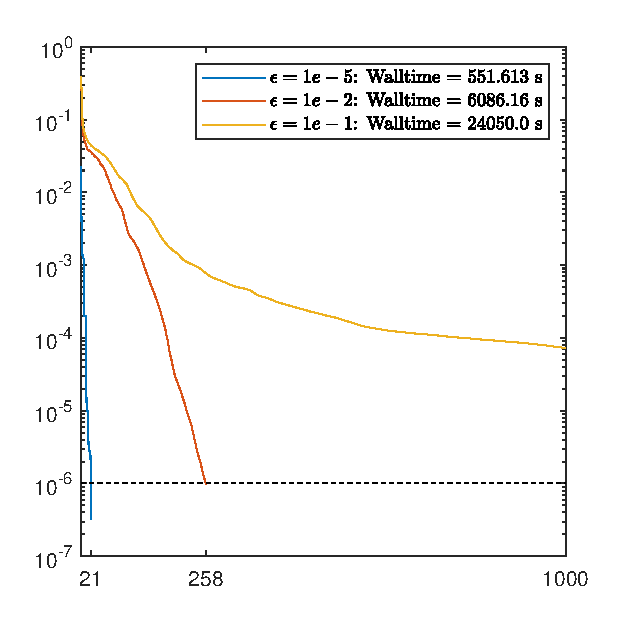
\includegraphics[width=0.5\textwidth]{Images/InitalGuessEPS.pdf}
    \caption{Convergence of the small rod problem with 3 different choices of epsilon. The $\epsilon = 1e-1$ problem did not converge in the given 1000 iterations.}
    \label{fig:InitalGuessEPS}
\end{figure}
Solving the problem for a smaller epsilon, however, does not give us an accurate initial guess for the actual problem with a larger epsilon, as the particle interactions are of a smaller magnitude. However, we note that the stokeslet matrix $A$ is dominated by the diagonal elements whose magnitude is proportional to $1/\epsilon$. If we consider two versions of the problem one with a smaller value of epsilon $\epsilon_1$ and stokeslet matrix $A_1$ and a target epsilon $\epsilon_2$ with a stokeslet matrix $A_2$ for which we would like to solve the problem. We first solve the initial problem with $\epsilon=\epsilon_1$, this should converge quickly in comparison to the second system and will return us a solution $\bm{F}_1$. The contribution to the first $3N_{F}$ terms are dominated by the diagonal elements of $\epsilon$ of order $1/\epsilon_1$ so by re-scaling the using a factor of $\epsilon_1/\epsilon_2$ we should have a better approximation to the solution. Very little has been published on the use of initial guesses with GMRES as often they provide little to no benefit to the overall computation. What is understood is the need for the residual from the initial guess $x_0$ to be lower than the residual of the right-hand side $b$ ($\lVert b-Ax_0 \rVert \leq \lVert r_o \rVert$). In order to achieve this, we use a trick outlined by Heged{\"u}s \cite{Saad1986GMRES:Systems,Strakos2005OnComputations} which minimises the residual using the method of least squares to obtain a scaling factor of 
\begin{equation*}
    \left\|r_{0}\right\|=\left\|b-A_2 \bm{F}_1 \zeta_{\min }\right\|=\min _{\zeta}\left\|b-A_2 \bm{F}_1 \zeta\right\|, \quad \zeta_{\min }=\frac{b^{T} A_2 \bm{F}_1}{\left\|A_2 \bm{F}_1\right\|^{2}}
    \label{eq:Hegedus}
\end{equation*}
where $\bm{F}_1$ is our initial guess from $A_2$ and our initial guess for the GMRES algorithm is $x_0 = \zeta_{\min} \bm{F}_1$. This initial guess gave some improvement in both cases as seen in \cref{tab:Preconditioning}.

\subsubsection{Rescaling Swimming Matrix} \label{sec:Rescale}
In the hope of cheaply reducing the condition of the matrix and more tightly clustering the eigenvalues of the swimming matrix, such that the GMRES algorithm converges in a smaller number of iterations \cite{CampbellGMRES}. We do this by rescaling the $B$ matrix in \cref{eq:swimmingStructure} such that its maximum value is one. This should reduce the condition of the matrix and cluster the eigenvalues at the centre. We are able to do this due to the $0$ force and moment constraints that we have imposed upon the problem and as such we are able to rescale our $B$ matrix without affecting the constraints. 
We do see a tighter clustering in the eigenvalues shown in \cref{appendix:ConNum} where the eigenvalues cluster closer to 1, however, the overall condition of the system increases.


\subsubsection{Preconditioning} \label{sec:Preconditioning}
A more optimal way in which we can solve Krylov subspace methods is to use a preconditioner such that the matrix system we are trying to solve has a smaller condition number with more clustered eigenvalues. This reduces the effect of small perturbations made by the GMRES method. If we call the swimming matrix defined in \cref{eq:swimmingStructure} $M$, the vector of unknowns $\bm{x}$ and the right hand side $\bm{b}$ then we can refer to the system as $Mx=b$. The matrix $M$ is significantly less well-conditioned (see \cref{appendix:ConNum}) than the stokeslet matrix $A$ and as such requires a significant number of iterations to solve.


Our preconditioner is based on work by Rostami and Olson \cite{Rostami2019FastBiofluids} and is inspired by the so-called “least-squares commutator” preconditioner \cite{Elman2005FiniteDynamics}. As described above we group the augmenting matrices into two larger matrices denoted $B$ and $B^\prime$. This means our swimming matrix can be written as 
\begin{equation*}
\begin{aligned}
\def\arraystretch{0.8}
    M = \left(\begin{array}{cc}
        A & B^\prime \\
        B & 0_{6N_{sw}\times6N_{sw}} 
    \end{array}\right) &= 
    \left(\begin{array}{cc}
        \mathds{1}_{3N_F \times 3N_F} & O_{3N_F\times6N_{sw}} \\
        BA^{-1} & \mathds{1}_{6N_{sw} \times 6N_{sw}}
    \end{array}\right)
    \left(\begin{array}{cc}
        A & B^\prime \\
        O_{6N_{sw}\times3N_F} & -BA^{-1}B^\prime
    \end{array}\right) \\
    &= LU.
\end{aligned}
\end{equation*}

This means $MU^{-1}$ has eigenvalues of 1 and as such GMRES should converge in one iteration \cite{Rostami2019FastBiofluids} if $U^{-1}$ is used as a right [hand side?] preconditioner to solve the system $MU^{-1}y = b$ where $x = U^{-1}y$. However due to the need to solve $BA^{-1}B^\prime$ this becomes infeasible, particularly when we do not construct $A$ explicitly.  Instead, we will attempt to cheaply approximate $U^{-1}$. We will denote the preconditioner matrix 
\begin{equation}
\def\arraystretch{0.8}
    P_M = \left(\begin{array}{cc}
        P_A & B^\prime \\
        O_{6N_{sw}\times3N_F} & P_S
    \end{array}\right)
    \label{eq:Precon}
\end{equation}
where $P_A$ is a preconditioner for the matrix $A$ and $P_S$ is a preconditioner for $-BA^{-1}B^\prime$. The Schur complement \cite{Zhang2005TheApplications,Lu2002InversesMatrices} allows us to compute the inverse of a $2 \times 2$ block matrix as 
\begin{equation*}
\def\arraystretch{0.8}
    \left(\begin{array}{cc}
        A & B \\
        C & D
    \end{array}\right)^{-1} = \left(\begin{array}{cc}
A^{-1}+A^{-1} B\left(D-C A^{-1} B\right)^{-1} C A^{-1} & -A^{-1} B\left(D-C A^{-1} B\right)^{-1} \\
-\left(D-C A^{-1} B\right)^{-1} C A^{-1} & \left(D-C A^{-1} B\right)^{-1}
\end{array}\right) 
\end{equation*}
if $A$ is invertible. This gives that the inverse of our preconditioner matrix \cref{eq:Precon} is
\begin{equation*}
\def\arraystretch{0.8}
        P_M^{-1} = \left(\begin{array}{cc}
        P_A^{-1} & -P_A^{-1} B^T P_S^{-1} \\
        O_{6N_{sw}\times3N_F} & P_S^{-1}
    \end{array}\right)
\end{equation*}
We, therefore, need to solve two systems of equations involving $P_A$ and one linear system involving $P_S$. As we stated above solving a linear system involving $P_S$ is too computationally challenging to form and solve, so we must look for an approximation to this solution. Inspired by the method of least squares we look for a solution $C$ which minimises the residual of $\lVert AB^T - B^\prime C \rVert \;\forall\; C \in \mathbb{R}^{6N_{sw}\times6N_{sw}}$. This solutions is found by taking the square of the residual to obtain $(AB^T - B^\prime C)^T(AB^T - B^\prime C) = (AB^T)^T(AB^T)-(AB^T)^TB^\prime C-C^T(B^\prime)^TA^T + C^T(B^\prime)^TB^\prime C$. Taking the derivative of this with respect to $C$ equal to $0$ will minimise the residual squared. This yields $-2(B^\prime)^TAB^T + 2(B^\prime)^TB^\prime C=0$ so $C = ((B^\prime)^TB^\prime)^{-1}(B^\prime)^TAB^T$. Computing the inverse of $C$ we get that $C^{-1} = ((B^\prime)^TAB^T)^{-1}((B^\prime)^TB^\prime)$. As we have minimised the residual we can say that $AB^T \approx B^\prime C \implies B^T C^{-1} = A^{-1}B^\prime$. Substituting both of these into our equation for our preconditioner $P_S$ gives us that, 
\begin{equation}
\begin{aligned}
    P_S = - B A^{-1}B^\prime &= -B B^{T} C^{-1} \\
    & = -(B B^{T})((B^\prime)^TAB^T)^{-1}((B^\prime)^TB^\prime) \\
    \implies P_S^{-1} &= -((B^\prime)^TB^\prime)^{-1}((B^\prime)^TAB^T)(B B^{T})^{-1}
\end{aligned}
\label{eq:PreconS}
\end{equation}
The computation of $P_S^{-1}$ now only involves solving the linear systems $(B^\prime)^TB^\prime$ and $B B^{T}$, however, these are cheap and easy to solve as both matrices are mainly sparse with dominant diagonal elements due to their construction. We still need to compute the solution to $P_A^{-1}$. We will consider solving this via a block diagonal form of the KIFMM where we only consider the interactions between nodes. 
The block diagonal preconditioner captures most of the dominant interactions between particles and provides a relatively accurate estimation of the solution to $A^{-1}$ and is significantly quicker to run. It also reduces the system to a set of simpler problems, one for each node. These are quicker and easier for GMRES to solve and, as such, the method can converge quicker for these systems. This principle could be extended to include all nodes in the $U$ interaction list, this provides better results for a single pass however due to the off-diagonal elements now being included, the problem is less well-conditioned with longer interaction times so we will only consider the purely block-diagonal preconditioner. Block diagonal preconditions have been used to solve problems in systems using the Rotne-Prager-Yamakawa (RPY) tensor \cite{UsabiagaHYDRODYNAMICSAPPROACH}, Stokeslet\cite{Nazockdast2017AMechanics} and more general elliptical PDEs \cite{Ibeid2018FastEquations}. 

Following on from using the diagonal preconditioner for $P_A^{-1}$ we will also consider a cheaper approximation to full matrix multiplication of $A$ in the computation of $P_S^{-1}$. Following on from the results shown in \cref{fig:QuadPoints} we note a  cheaper but less accurate computation can be achieved by using fewer quadrature points for the equivalent surfaces, in this way, 60 quadrature points were chosen as it provided a good balance between the accuracy of the method and provides a noticeable speed increase compared to the full method with 152 quadrature points. 

\subsection{Results}



The results of all 3 optimisations can be seen in \cref{tab:Preconditioning} along with data for the non preconditioned system. All methods had a fixed stopping criterion of $\lVert Mx-b \rVert_2/\lVert b \rVert_2 \leq 10^{-6}$ as is the default in MATLAB's GMRES method. The 2016 swimmer model proved challenging to solve with over 150 more GMRES iterations needed to converge to the same tolerance when no preconditioner was used. Both methods were aided by the use of an initial guess with the computation time being reduced by nearly 10\% as the initial iterations are replaced by quicker iterations using a smaller $\epsilon$ value. The attempt at re-scaling the lower augmented matrix was proven to increase the overall computation time, where the tighter clustered eigenvalues did not allow the method to converge any quicker. More work could be done in order to find a correct scaling factor to keep the tightly clustered eigenvalues and reduce the overall condition of the matrix. 

\begin{table}
\begin{singlespace}
\centering
\setlength{\tabcolsep}{6pt}
\renewcommand{\arraystretch}{1.4}
\caption{Comparison of preconditioners in the case of Rods in Shear Flow. All methods converged to a relative residual error smaller than $10^{-6}$}
\small
\begin{tabular}{p{2cm} p{1cm} p{2cm} p{1.5cm} p{0.1cm} p{1cm} p{2cm} p{1.5cm}}
\multirow{2}{*}{\parbox{1.8cm}{number of swimmers}} & \multicolumn{3}{l}{No precondtioner} & & \multicolumn{3}{l}{Initial Guess} \\ \cline{2-4} \cline{6-8}
  & \# of iters & \# of MVPs ($M$) & walltime (sec.) & & \# of iters & \# of MVPs ($M_{\epsilon_1}/M_{\epsilon_2}$) & walltime (sec.) \\ \hline
  203 & 250 & 250 & 8599 & &  268 & 20/248 & 7763\\
  2016 & 409 & 409 & 23645 & & 358 & 12/346 & 20977\\ \hline
  \multirow{2}{*}{\parbox{1.8cm}{number of swimmers}} & \multicolumn{3}{l}{Rescaling} & &\multicolumn{3}{l}{Least-squares commutator} \\ \cline{2-4} \cline{6-8}
  & \# of iters & \# of MVPs ($M$) & walltime (sec.) & & \# of iters & \# of MVPs ($M/P_A^{-1}/A_S$) & walltime (sec.) \\ \hline
  203 & 297 & 297 & 9357 & & 71 & 62/124/63 & 3739 \\
  2016 & 523 & 523 & 34036 & & 47 & 47/96/48 & 4165 
\end{tabular}
\label{tab:Preconditioning}
\end{singlespace}
\end{table}

As expected, preconditioning of the system proved most effective in reducing the overall computation time, particularly with the 2016 swimmer case where the computation time drops by 80\%. The 203 swimmer case does not see such a significant drop with a decrease in computation time of 50\%, possibly due to the larger contribution that the stokeslet matrix $A$ has on the computation. We would expect to see that, for systems with more swimmers and the same number of quadrature points, the number of GMRES iterations needed to converge would stay approximately the same, and as such, larger systems could be tackled. Combinations of these methods may prove useful in reducing the calculation further, such as initial guesses for preconditioned systems, however, due to the rapid decrease in the residual from the preconditioned system it is doubtful that it will provide any noticeable gain and the need to use the Heged{\"u}s trick involves another full matrix product.

\begin{table}
\begin{singlespace}
\centering
\setlength{\tabcolsep}{6pt}
\renewcommand{\arraystretch}{1.4}
\caption[The use of hybrid KIFMM NEAREST method to solve the 2016 rod case.]{The use of hybrid KIFMM NEAREST method to solve the 2016 rod case. Both preconditioned and not preconditioned methods converged to a relative residual error smaller than $10^{-6}$ of the Joint case. Neither system converged in the maximum 1000 iterations for the Disjoint case.}
\small
\begin{tabular}{p{2cm} p{0.75cm} p{2cm} p{1.0cm} p{0.1cm} p{0.75cm} p{2.5cm} p{1.5cm}}
\multirow{2}{*}{\parbox{1.8cm}{NEAREST Spacing}} & \multicolumn{3}{l}{No precondtioner} & & \multicolumn{3}{l}{Least-squares commutator} \\ \cline{2-4} \cline{6-8}
  & \# of iters & \# of MVPs ($M$) & walltime (sec.) & & \# of iters & \# of MVPs ($M/P_A^{-1}/A_S$) & walltime (sec.) \\ \hline
  Joint & 201 & 201 & 2898 & &  47 & 47/96/48 & 1394\\
  Disjoint & 1000 & 1000 & 10436 & & 1000 & 1000/2002/1001 & 19734
\end{tabular}
\label{tab:PreconditioningNear}
\end{singlespace}
\end{table}

In order to evaluate the use of the hybrid KIFMM NEAREST method we solved the swimming problem for the case of 2016 in a shear flow. In order to compare between non NEAREST and NEAREST computations we discretise each spheroid with 42 fine quadrature points matching the discretisation in the non-nearest case and introduce a coarse discretisation with spacing 2 times larger such that the surface is discretised by 12 force quadrature points.  This gives a total of 72576 SDOF for each system with 84672 and 108864 fine quadrature points for the joint and disjoint cases respectively. Although results will differ slightly based on \cref{fig:NEARESTCOMPFMM,fig:NEARESTCOMP} and data collected by Smith \cite{Smith2018AEquation} show that the overall difference will be small. Figure \ref{tab:PreconditioningNear} shows that we see a large increase in performance for the joint case with a 2.7$\times$ speed up in the computation for the preconditioned system. The overall increase in speed found obtained by using a preconditioner is only 2$\times$ compared to the 5$\times$ speed up found in the non NEAREST computations. Results for the Disjoint case are less promising with neither simulation converging in 1000 iterations. The convergence rate of both systems appears to stagnate early with the pre-conditioned system failing to converge to a residual error of $4\times 10^{-2}$. This is due to the choice of the block-diagonal preconditioner which does not represent the system as closely as it does for other discretisation. 

\begin{figure}
    \centering
    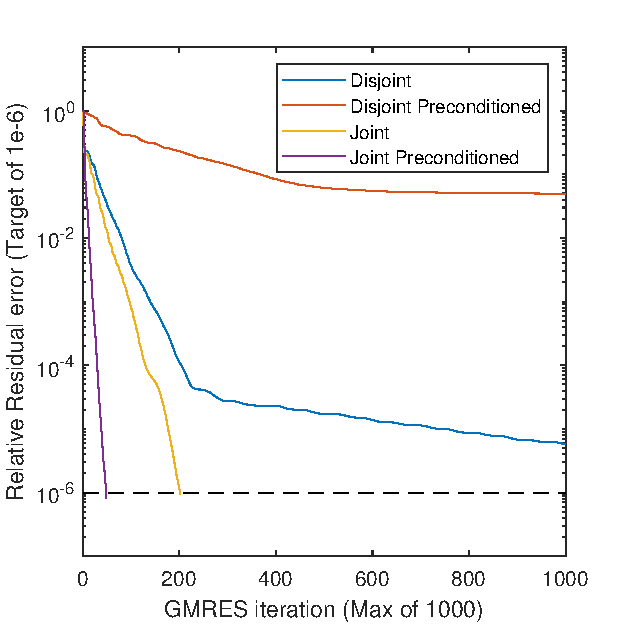
\includegraphics[width=0.5\textwidth]{Images/Rods/NearestPrecon.pdf}
    \caption{Convergence rate of NEAREST discretisation when used to solve the rods in a shear flow problem.}
    \label{fig:NearestConverge}
\end{figure}

\subsection{Squirmers}
The slip velocity spherical squirmier is used widely in models of propulsion in stokes flow \cite{Smith2021TheSelf-Propulsion,Lauga2020TheModel,Pedley2016SquirmersSwimming}. The squirmer model allows for the representation of swimming motion generated by many beating cilia without the need to simulate each cilium individually. By scaling the coordinate system such that the radius of the spherical squirmer is 1, we denote an angle relative to the north pole as $\theta$ which lies between $0\leq\theta\leq\pi$. We also define $\bm{t}(\theta)$ to be the tangent to the sphere pointing towards the south pole. Then the velocity in the body frame of the the squirmier is $\bm{u}(\theta) = sin(\theta)\bm{t}(\theta)$ as seen in \cref{fig:Squiremer3D}. We also plot the streamlines around the squirmers in \cref{fig:Squiremer3DFlow}, where the force at each force discretisation point on the squirmier is solved through the resistance problem. In order to refine the accuracy of the flow field, the hybrid NEAREST method was used with 3756 SDOF based on 1252 force quadrature points and 20058 fine quadrature points. The force field was then evaluated on a Cartesian grid in the domain $[-2\; 2] \times [-2\; 2] \times [-2\; 2]$ with a total of 125000 evaluation points. 

\begin{figure}
\begin{subfigure}[b]{0.4\textwidth}
    \centering
    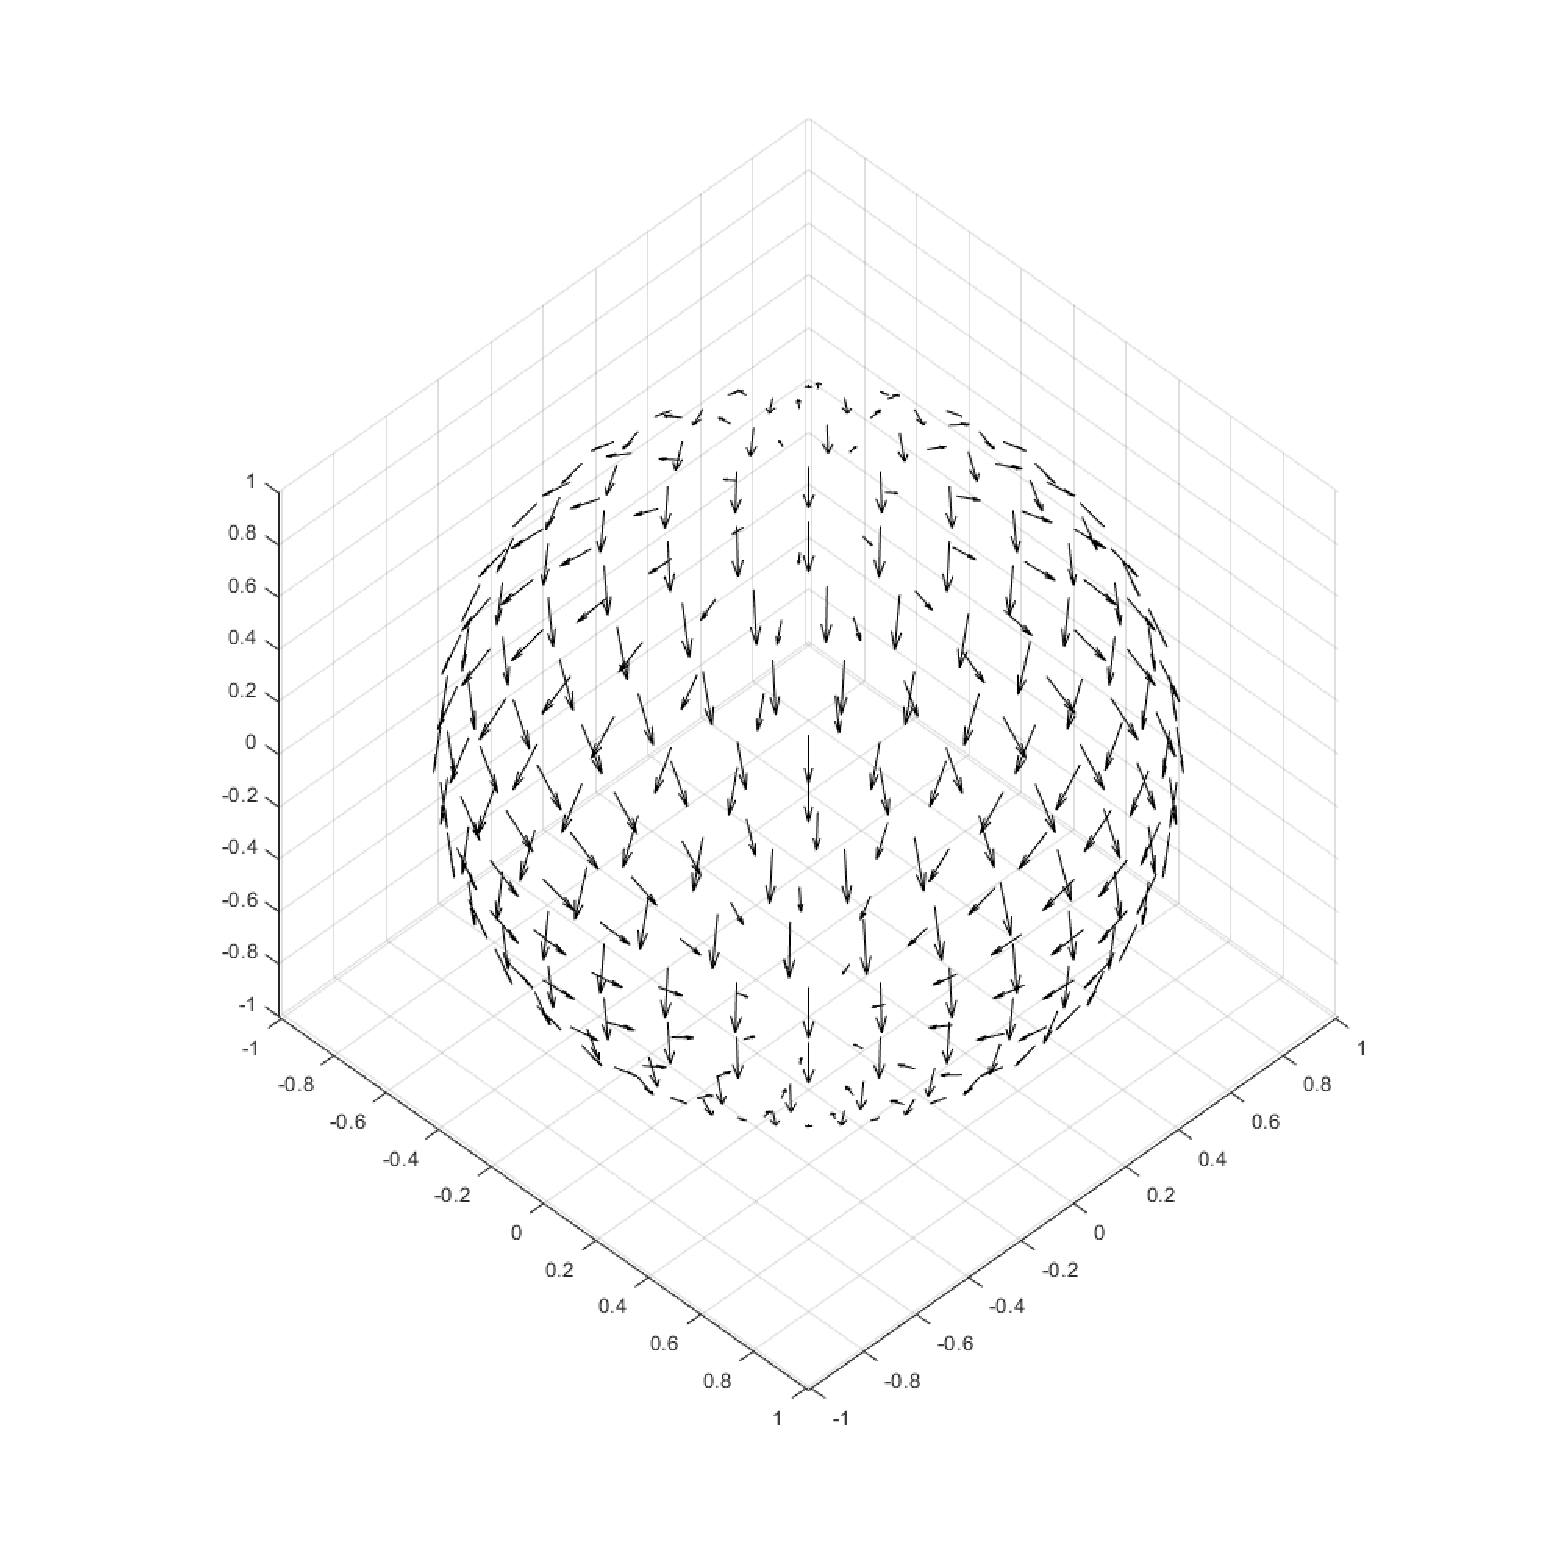
\includegraphics[width=\textwidth]{Images/squirmers/Squiremer3D.pdf}
    \caption[]{\label{fig:Squiremer3D}}
\end{subfigure}
\hfill
\begin{subfigure}[b]{0.4\textwidth}
    \centering
    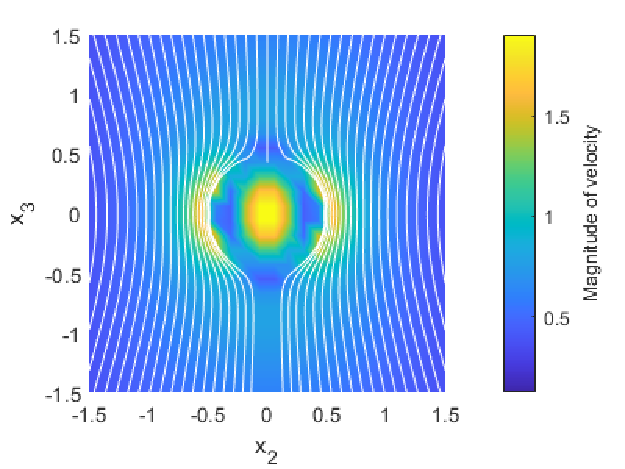
\includegraphics[width=\textwidth]{Images/squirmers/StreamLinesSingle.pdf}
    \caption[]{\label{fig:Squiremer3DFlow}}
\end{subfigure}
\caption[Velocity and Streamlines flow around a single squirmer.]{(i) Graph showing the magnitude of the velocity on the surface of a single squirmer. (ii) The computed velocity profile with streamlines in the $(x_2,x_3)$ plane}
\end{figure}

The interactions of multiple squirmers are considered in \cref{fig:Squiremer3DFlowPair} where we first solve a swimming problem, each swimmer is discretised with 1252 force quadrature points and 20058 fine quadrature points, totalling 7524 SDOF for each swimming problem. Noting that $\bm{b}^{(3)} = \bm{b}^{(1)} \times \bm{b}^{(2)}$ we only need to return the changes in the first two basis vectors, At each time step we return 
\begin{equation*}
    {\dot{\bm{x}}}_{0}=\bm{U}\left(\bm{x}_{0}, \bm{b}^{(1)}, \bm{b}^{(2)}, t\right), \quad \dot{\bm{b}}^{(j)}=\bm{\Omega}\left(\bm{x}_{0}, \bm{b}^{(1)}, \bm{b}^{(2)}, t\right) \times \bm{b}^{(j)}, \quad j=1,2
\end{equation*}
in the form
\begin{equation*}
\arraycolsep=0.4pt\def\arraystretch{1}
\dot{Y} = \begin{bmatrix}
    {\dot{\bm{x}}_{0 j}} \\
    {\dot{\bm{b}}^{(1)}}_j \\
    {\dot{\bm{b}}^{(2)}}_j
\end{bmatrix} \quad \text{ for } j=1,..,N_{sw}
\end{equation*}
The problem is then formulated by a set of $9 \times N_{sw}$ differential equations which can be solved using Matlab's ode45 solver. The resistance problem is then solved for the needed time steps and the velocity is evaluated on a cartesian grid in the domain $[-3\; 3] \times [-3\; 3] \times [-3\; 3]$ with a total of 125000 evaluation points. Figure \ref{fig:Squiremer3DFlowPair} shows the flow field at select time steps during the simulation. A regularisation parameter of $10^{-2}$ was chosen such the condition of the Resistance problem was relatively low and a fine quadrature spacing of a quarter of the force spacing was used as recommended by Smith and Gallagher \cite{Gallagher2020}.  

\begin{figure}
\centering
\begin{subfigure}[b]{0.22\textwidth}
    \centering
    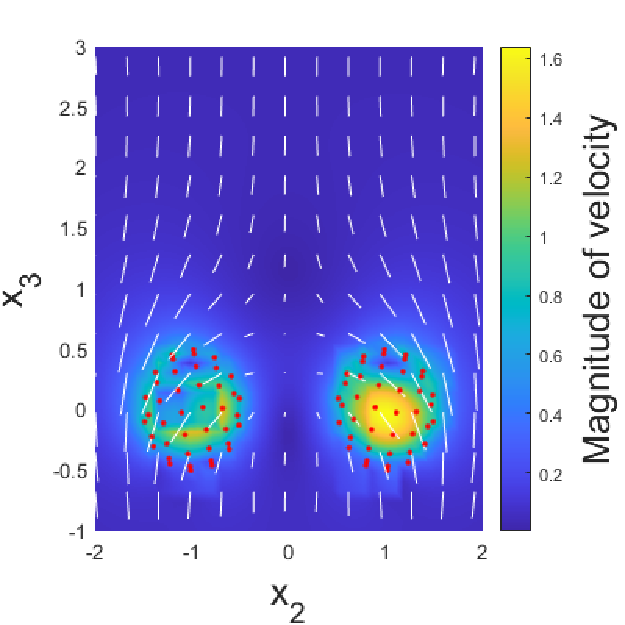
\includegraphics[width=\textwidth]{Images/squirmers/Pair-1.pdf}
    \caption[]{\label{fig:PairA}}
\end{subfigure}
\begin{subfigure}[b]{0.22\textwidth}
    \centering
    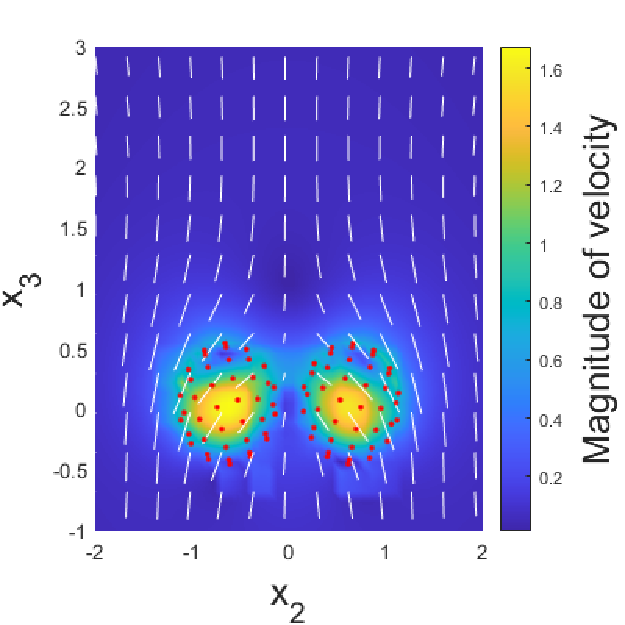
\includegraphics[width=\textwidth]{Images/squirmers/Pair-2.pdf}
    \caption[]{\label{fig:PairB}}
\end{subfigure}
\begin{subfigure}[b]{0.22\textwidth}
    \centering
    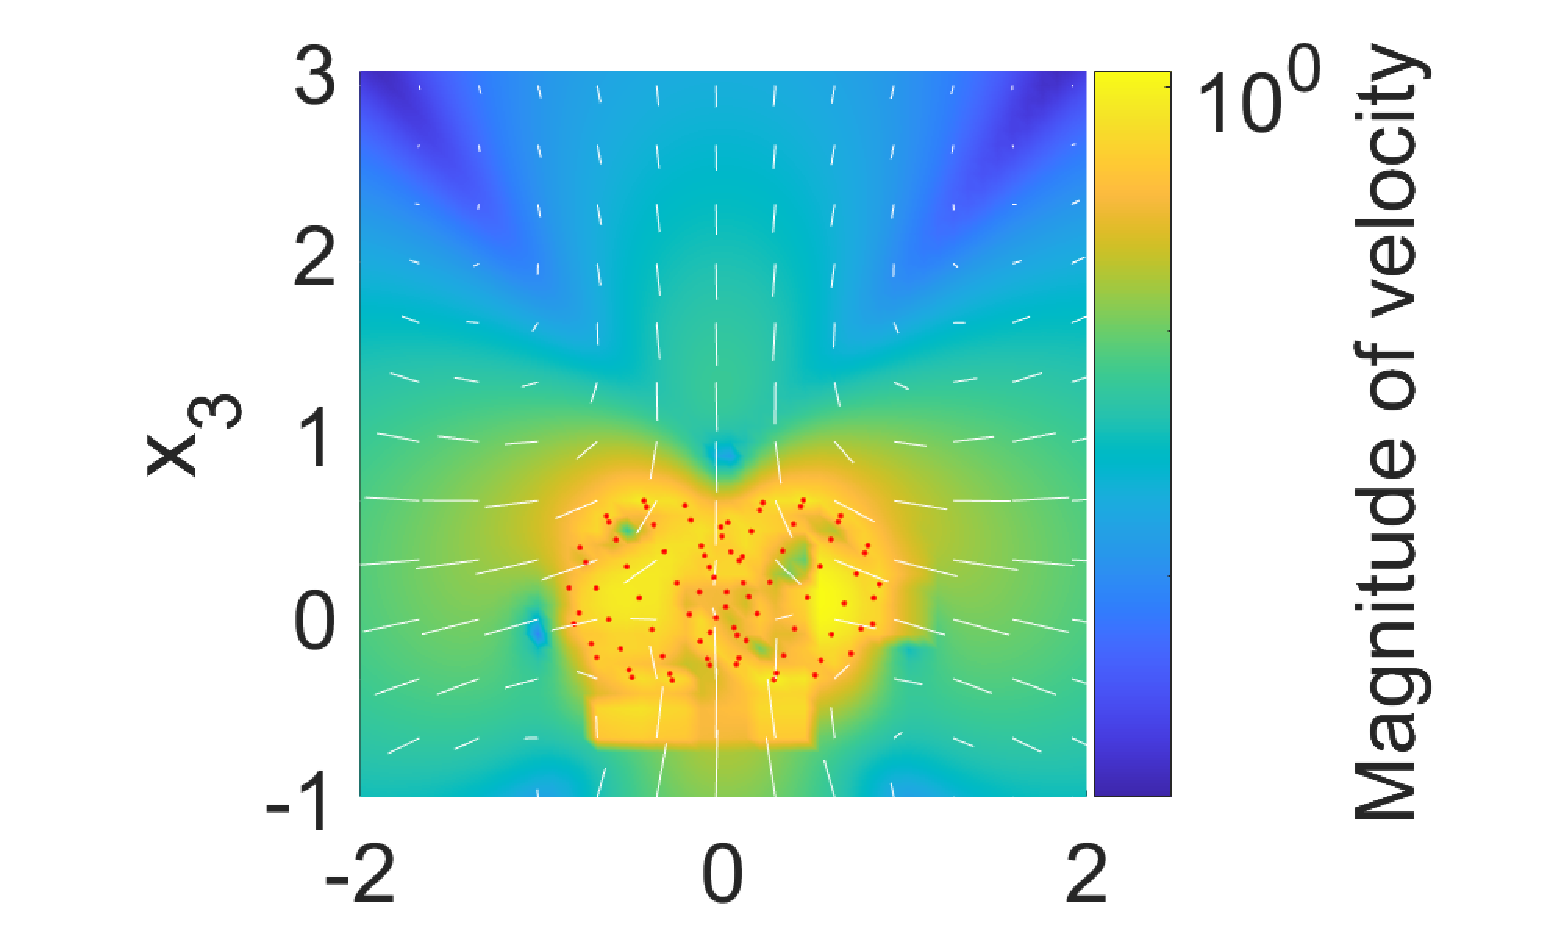
\includegraphics[width=\textwidth]{Images/squirmers/Pair-3.pdf}
    \caption[]{\label{fig:PairC}}
\end{subfigure}
\begin{subfigure}[b]{0.22\textwidth}
    \centering
    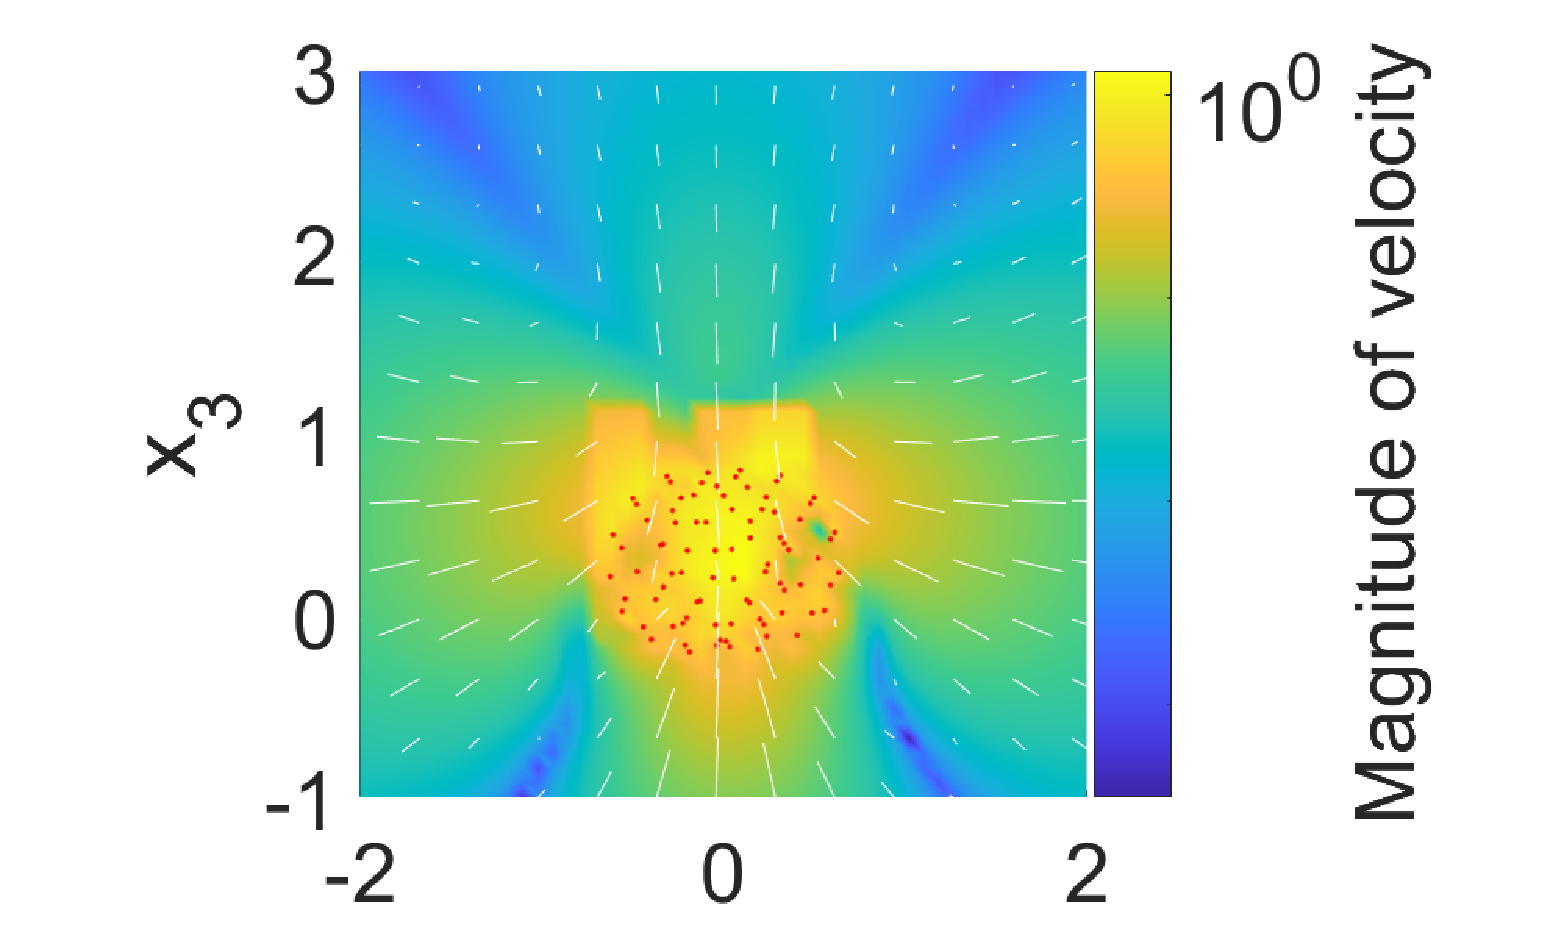
\includegraphics[width=\textwidth]{Images/squirmers/Pair-4.pdf}
    \caption[]{\label{fig:PairD}}
\end{subfigure}
\vskip\baselineskip
\begin{subfigure}[b]{0.22\textwidth}
    \centering
    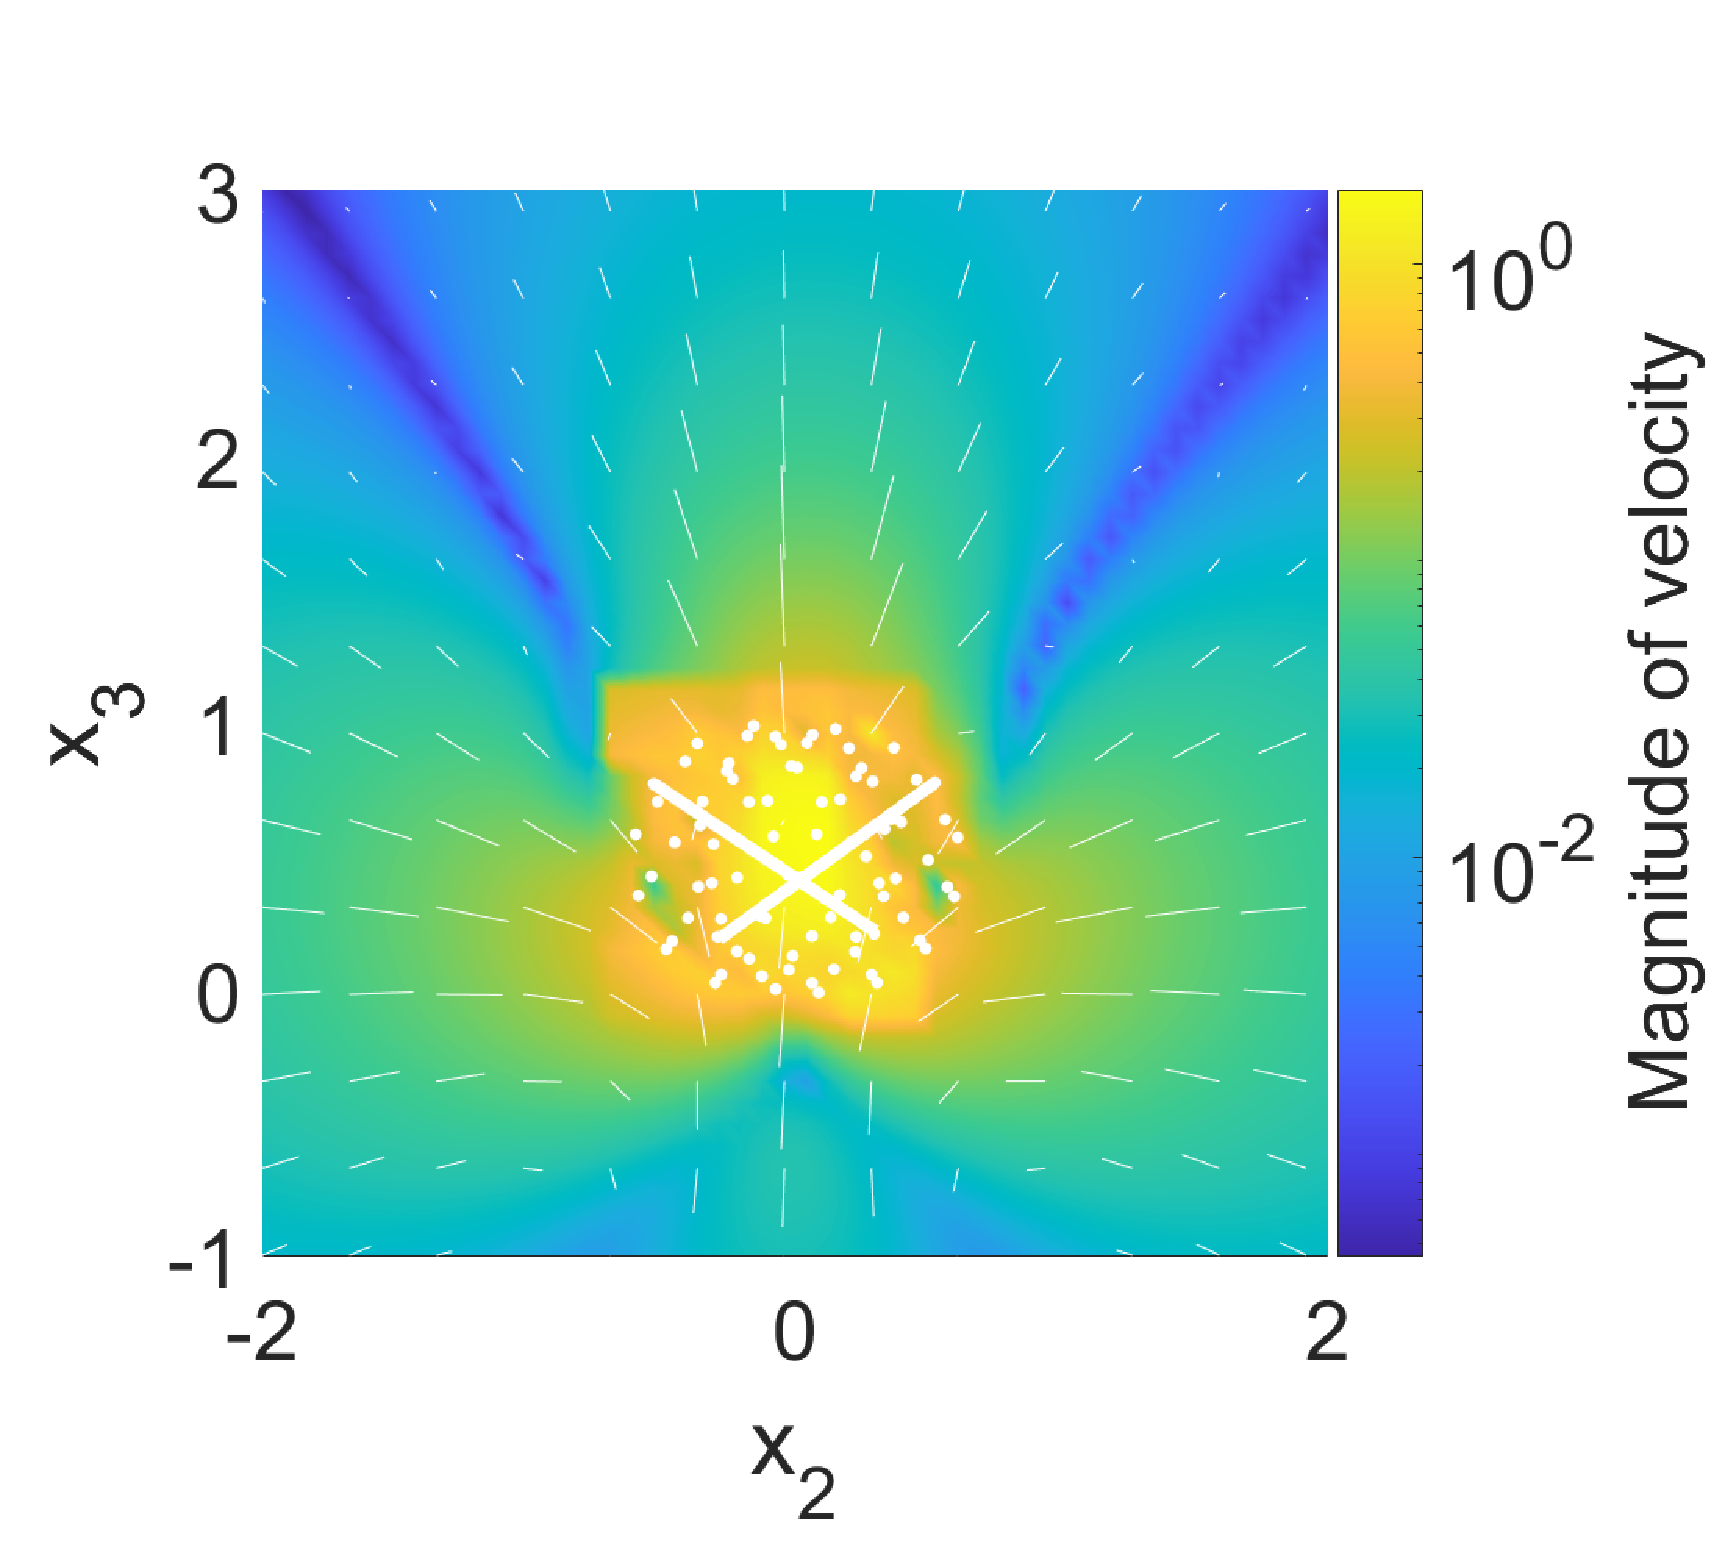
\includegraphics[width=\textwidth]{Images/squirmers/Pair-5.pdf}
    \caption[]{\label{fig:PairE}}
\end{subfigure}
\begin{subfigure}[b]{0.22\textwidth}
    \centering
    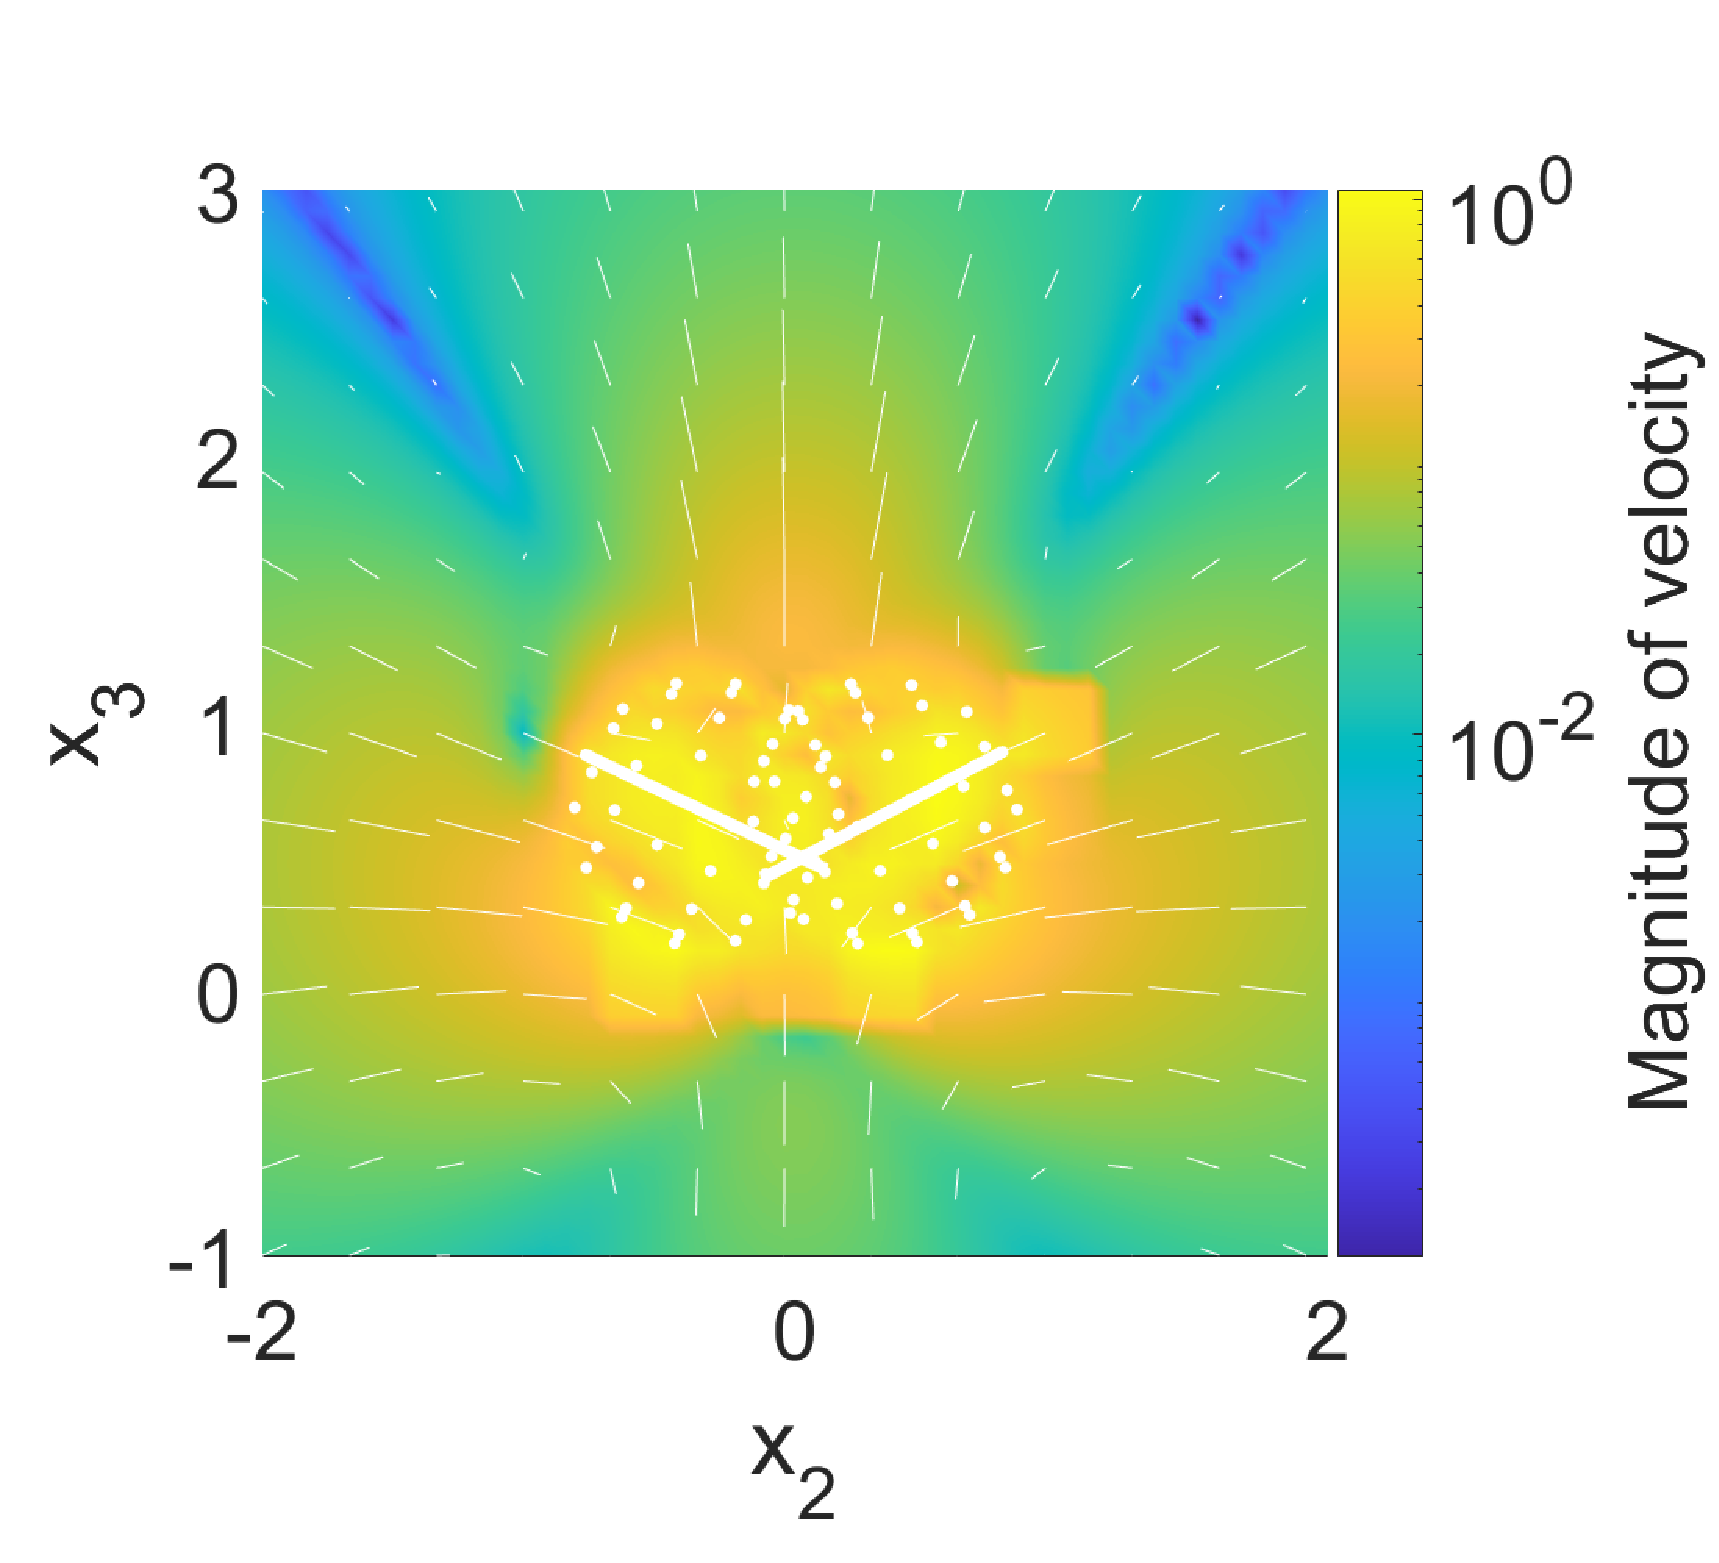
\includegraphics[width=\textwidth]{Images/squirmers/Pair-6.pdf}
    \caption[]{\label{fig:PairF}}
\end{subfigure}
\begin{subfigure}[b]{0.22\textwidth}
    \centering
    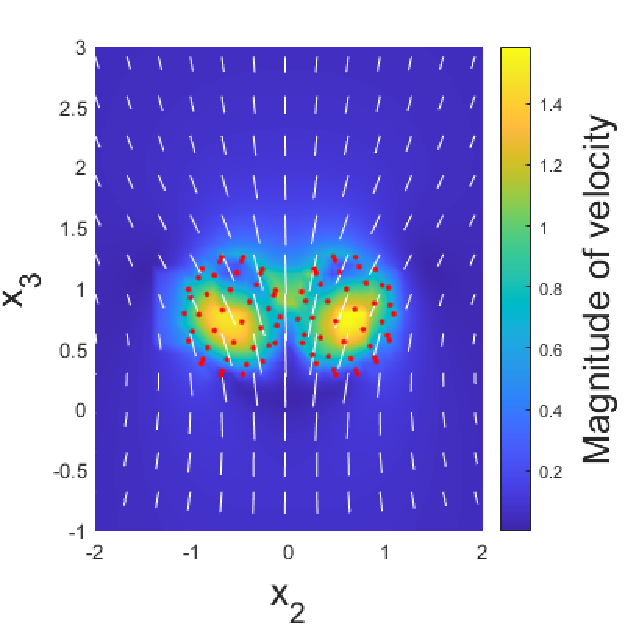
\includegraphics[width=\textwidth]{Images/squirmers/Pair-7.pdf}
    \caption[]{\label{fig:PairG}}
\end{subfigure}
\begin{subfigure}[b]{0.22\textwidth}
    \centering
    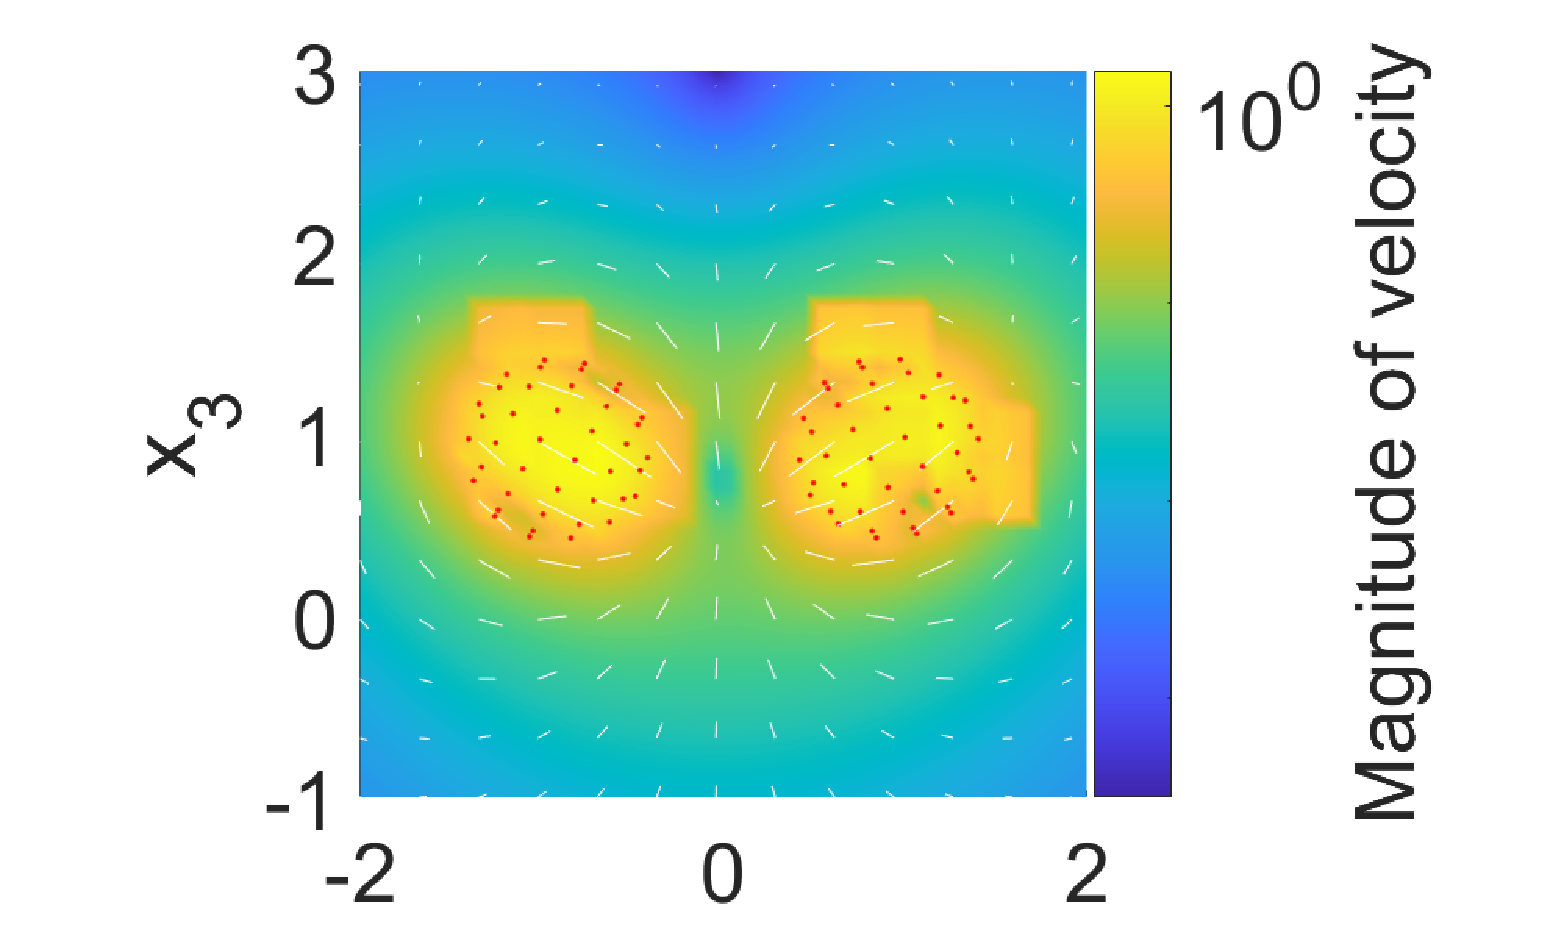
\includegraphics[width=\textwidth]{Images/squirmers/Pair-8.pdf}
    \caption[]{\label{fig:PairH}}
\end{subfigure}
\caption[Streamlines flows around a pair of squirmers.]{\label{fig:Squiremer3DFlowPair}Streamlines flows around a pair of squirmers at various time steps. The coarse discretisation points of the squiremer are plotted in red. (i-viii) are taken at slices in the simulation at times t = 0, 0.14, 0.29, 0.49, 0.57, 0.71, 0.86 and 1 respectively.}
\end{figure}

\subsubsection{Bottom heavy squirmers}
For larger simulations, the choice was made to study bottom-heavy squirmers in a gravitational field \cite{Ruhle2020EmergentGravity,BrumleyStabilitySquirmers,Pedley2016SphericalMicro-organisms}. It has been seen that bottom-heavy squirmers, where the centre of mass lies below the geometric centre of the sphere, form clusters which rise and fall when confined between two parallel plates \cite{Ruhle2020EmergentGravity}. Implantation of both gravity and bottom heaviness is easy due to the formulation of the swimming problem, we set $\bm{G}=[0,0,g]$ where $g$ is the strength of gravity in the  direction. The torque is therefore defined to be $\bm{T}_j =  m g r_0 ( -\bm{b}_j^{(3)} \times \bm{e}_z)$ for $j=1,...,N_{sw}$ where $m$ is the mass of the squirmer (taken to be 1), $r_0$ is the offset of the centre of mass from the geometric centre and $\bm{e_z}$ is a unit vector pointing in the positive z-direction. We scatter 50 squirmers of radius $0.5$ in the region $[-1.6\; 1.6] \times [-1.6\; 1.6] \times [1\; 4.5]$. Each squirmer starts in a random direction and with a maximum velocity of two on the equator of the sphere. In order to constrain the squirmers we define two walls one at $z=0$ and the other at $z=10$ each with a size of $10 \times 10$. In order to keep the total scalar degrees of freedom reasonable 26 force points and 206 fine quadrature points are placed over the surface of the sphere with an effective spacing of 0.33 and 0.1 respectively. The boundaries are discretised with 3808 force points and 62382 fine quadrature points with effective spacing of 0.25 and 0.0625 respectively. 

\begin{figure}
\centering
\begin{subfigure}[b]{0.22\textwidth}
    \centering
    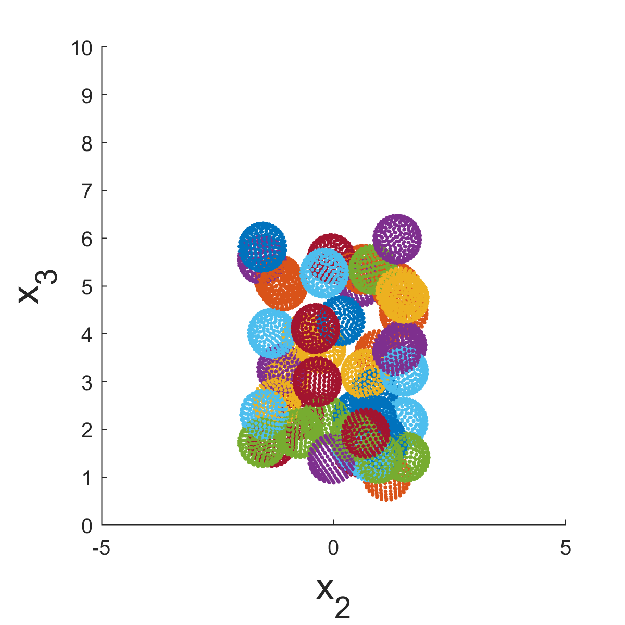
\includegraphics[width=\textwidth]{Images/squirmers/Gyro-1-All.pdf}
    \caption[]{\label{fig:squirmerPosA}}
\end{subfigure}
\begin{subfigure}[b]{0.22\textwidth}
    \centering
    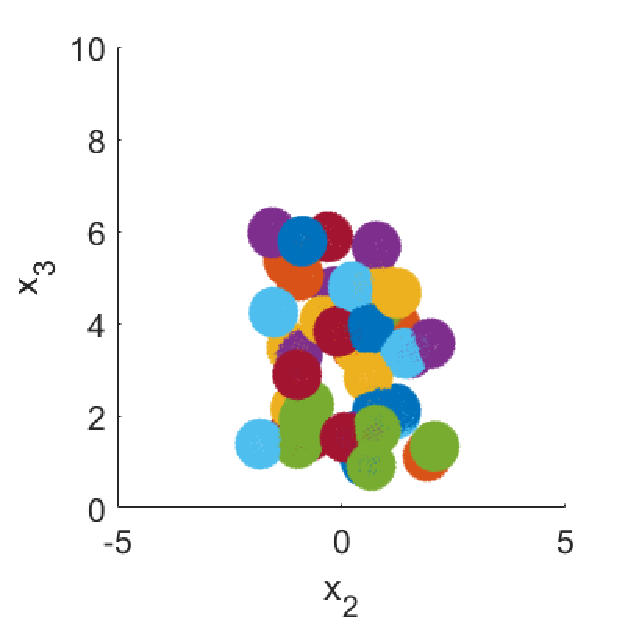
\includegraphics[width=\textwidth]{Images/squirmers/Gyro-2-All.pdf}
    \caption[]{\label{fig:squirmerPosB}}
\end{subfigure}
\begin{subfigure}[b]{0.22\textwidth}
    \centering
    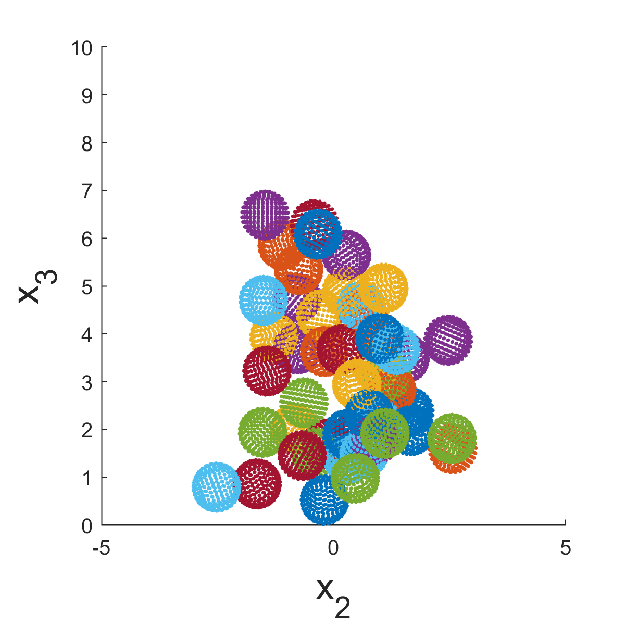
\includegraphics[width=\textwidth]{Images/squirmers/Gyro-3-All.pdf}
    \caption[]{\label{fig:squirmerPosC}}
\end{subfigure}
\begin{subfigure}[b]{0.22\textwidth}
    \centering
    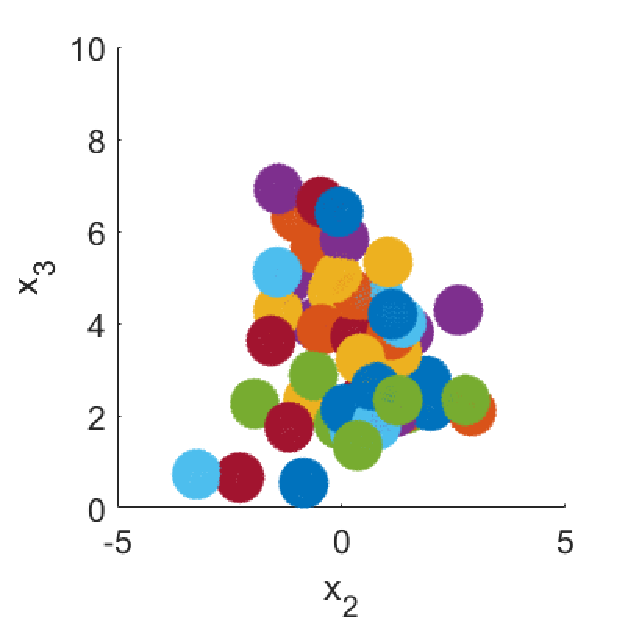
\includegraphics[width=\textwidth]{Images/squirmers/Gyro-4-All.pdf}
    \caption[]{\label{fig:squirmerPosD}}
\end{subfigure}
\vskip\baselineskip
\begin{subfigure}[b]{0.22\textwidth}
    \centering
    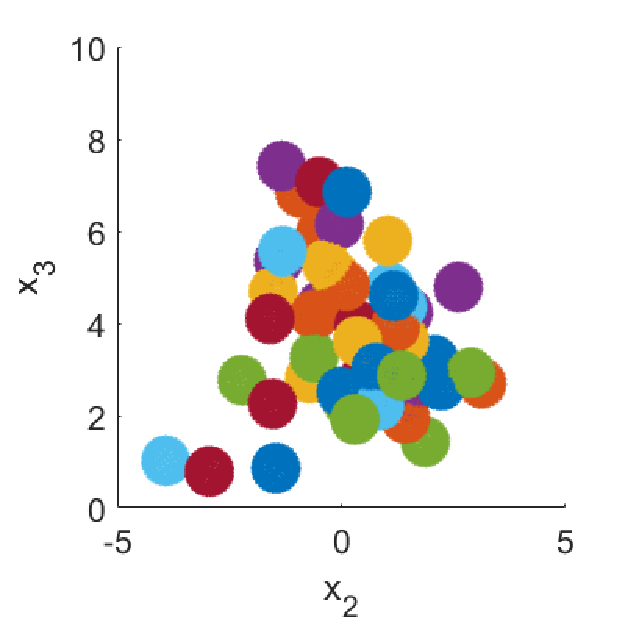
\includegraphics[width=\textwidth]{Images/squirmers/Gyro-5-All.pdf}
    \caption[]{\label{fig:squirmerPosE}}
\end{subfigure}
\begin{subfigure}[b]{0.22\textwidth}
    \centering
    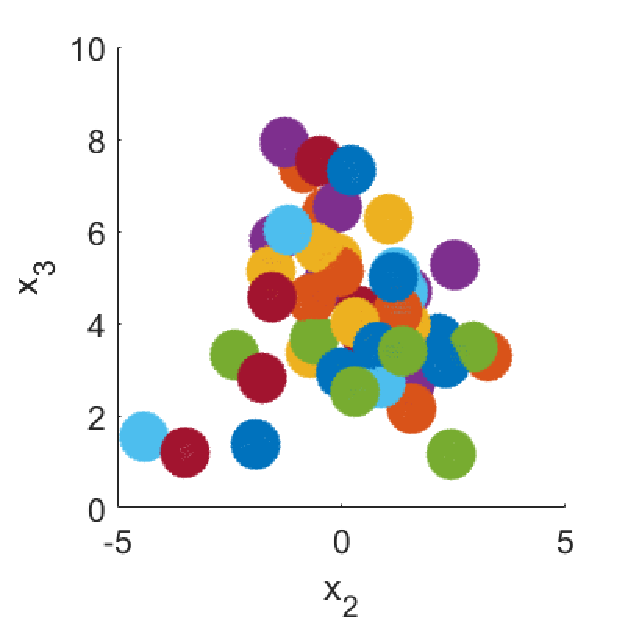
\includegraphics[width=\textwidth]{Images/squirmers/Gyro-6-All.pdf}
    \caption[]{\label{fig:squirmerPosF}}
\end{subfigure}
\begin{subfigure}[b]{0.22\textwidth}
    \centering
    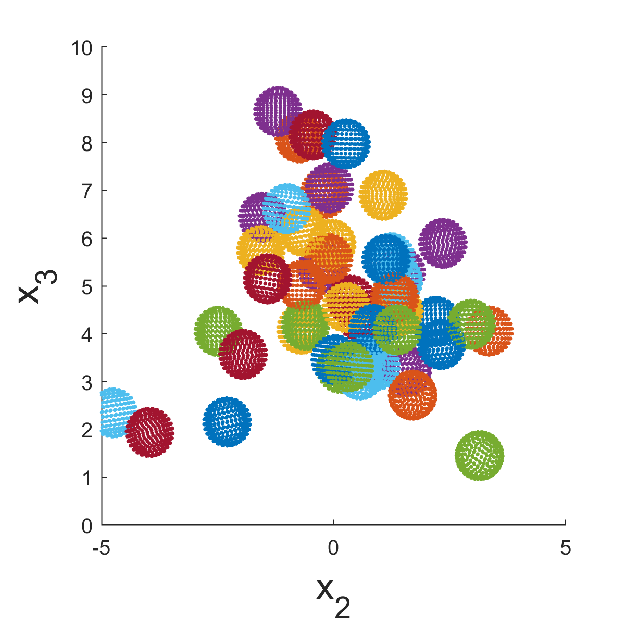
\includegraphics[width=\textwidth]{Images/squirmers/Gyro-7-All.pdf}
    \caption[]{\label{fig:squirmerPosG}}
\end{subfigure}
\begin{subfigure}[b]{0.22\textwidth}
    \centering
    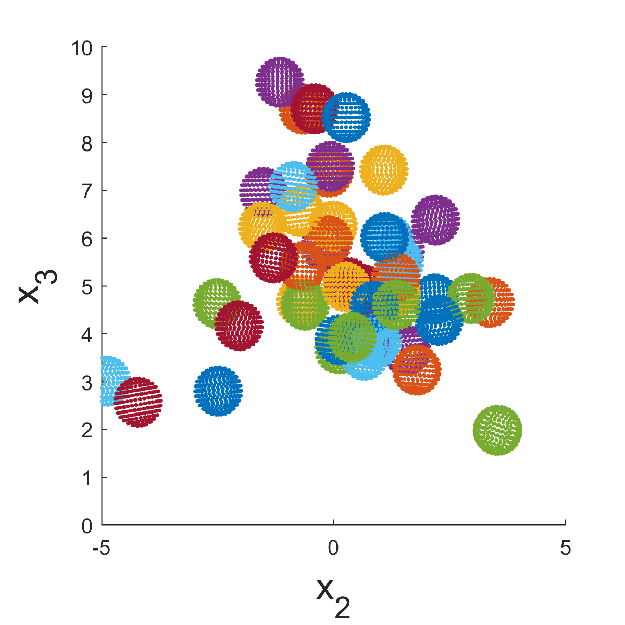
\includegraphics[width=\textwidth]{Images/squirmers/Gyro-8-All.pdf}
    \caption[]{\label{fig:squirmerPosH}}
\end{subfigure}
\label{fig:SquiremerGyroPo}
\caption[Position at 8 time steps of 50 squiremers randomly distributed at t=0.]{Position at 8 time steps of 50 squirmers randomly distributed at t=0. Two plates define the top and bottom of the simulations at $x_3 = 0$ and  $x_3 = 10$. (i-viii) show squirmer positions at t = 0, 0.74, 1.48, 2.212, 2.96, 3.70, 4.44 and 5.18 respectively.}
\end{figure}

\begin{figure}
\centering
\begin{subfigure}[b]{0.22\textwidth}
    \centering
    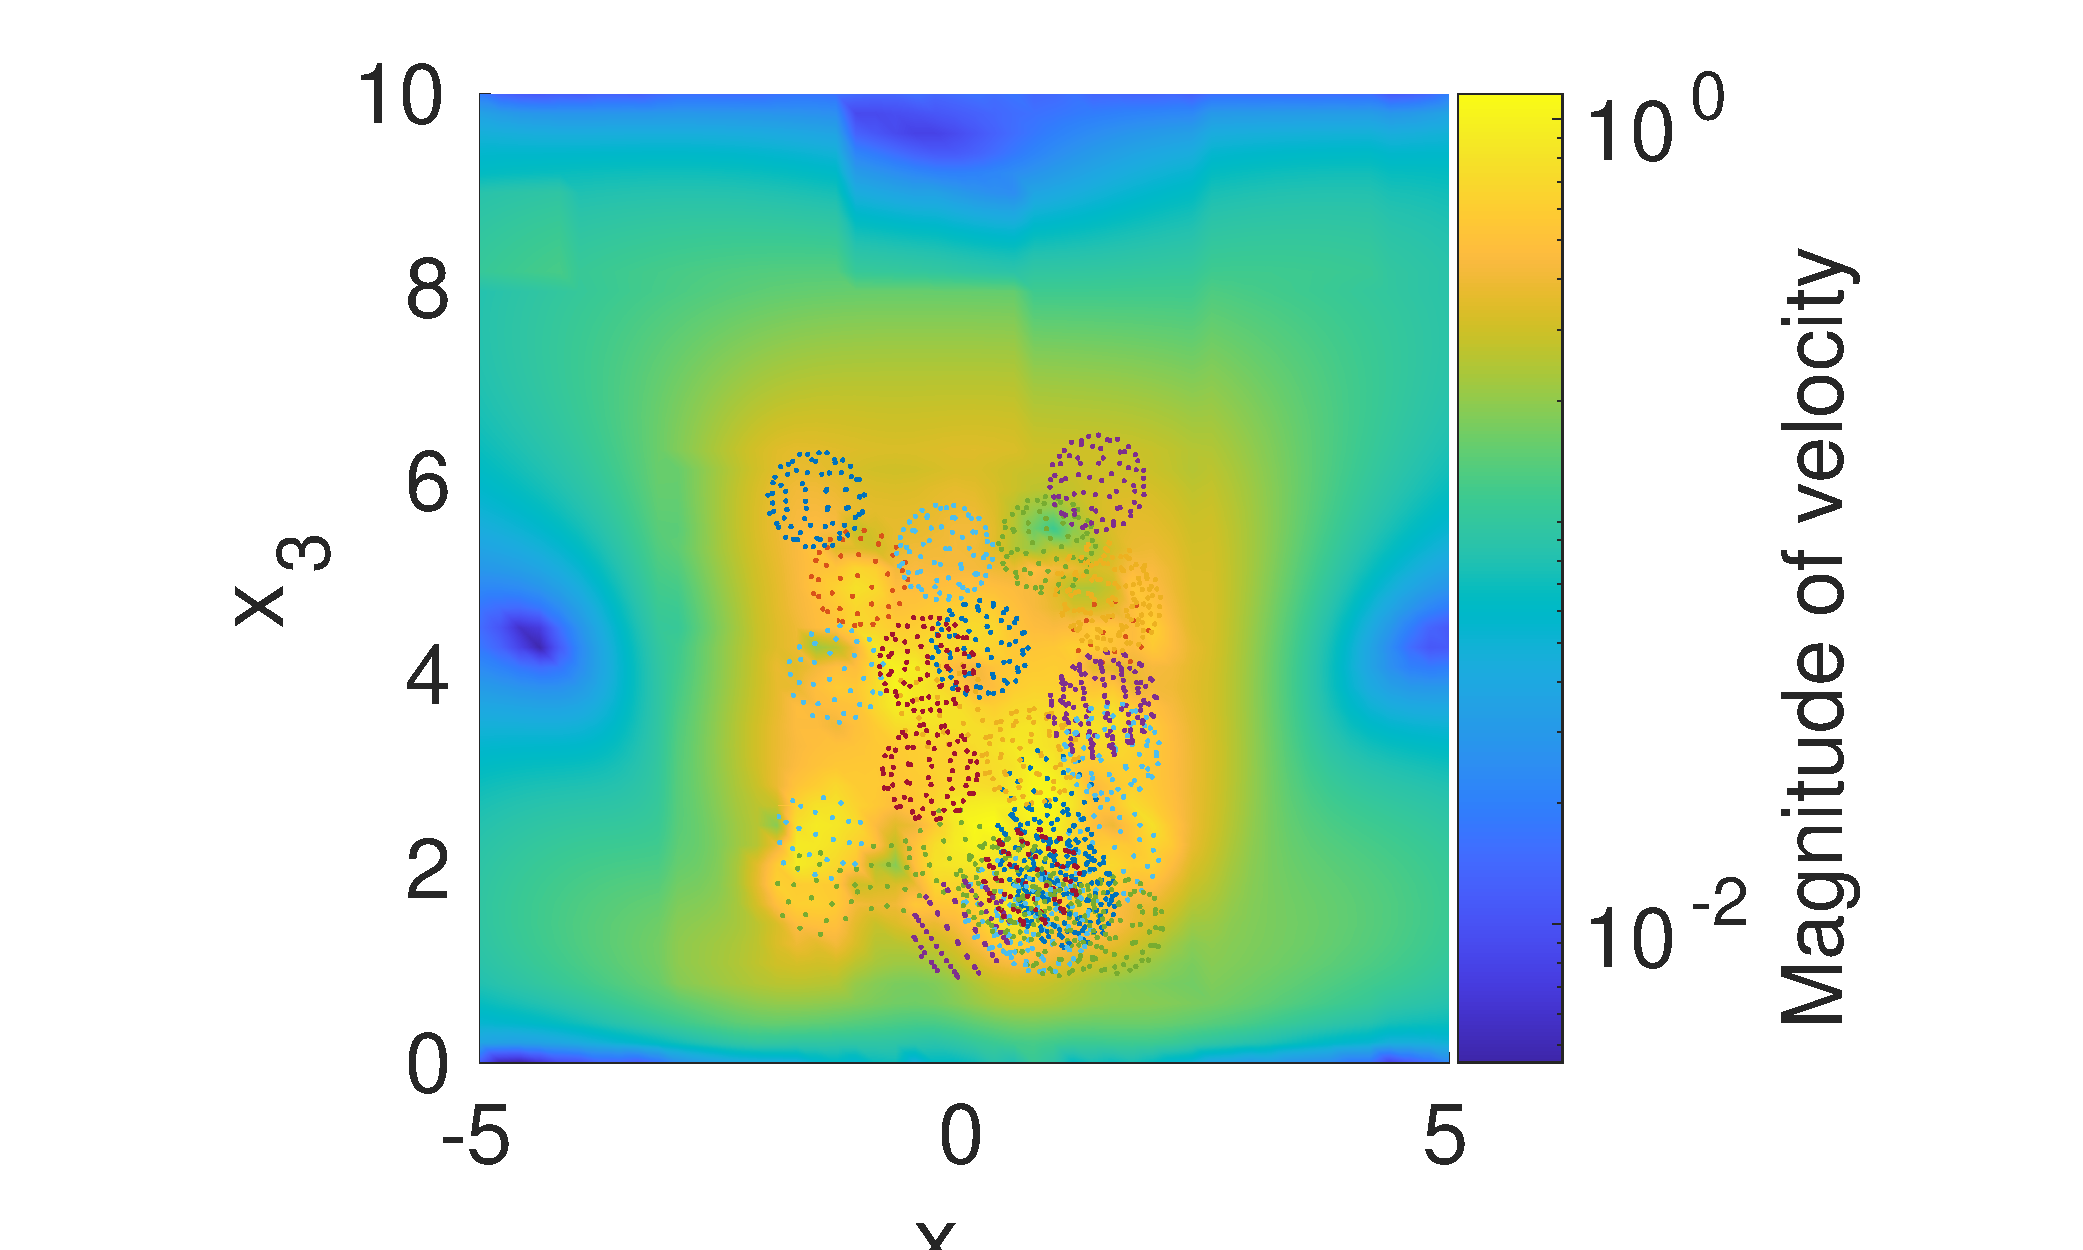
\includegraphics[width=\textwidth]{Images/squirmers/Gyro-1.pdf}
    \caption[]{\label{fig:squirmerA}}
\end{subfigure}
\begin{subfigure}[b]{0.22\textwidth}
    \centering
    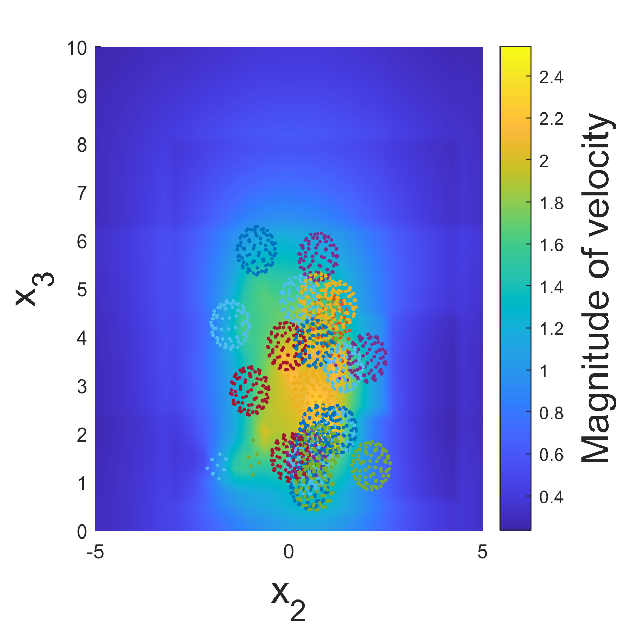
\includegraphics[width=\textwidth]{Images/squirmers/Gyro-2.pdf}
    \caption[]{\label{fig:squirmerB}}
\end{subfigure}
\begin{subfigure}[b]{0.22\textwidth}
    \centering
    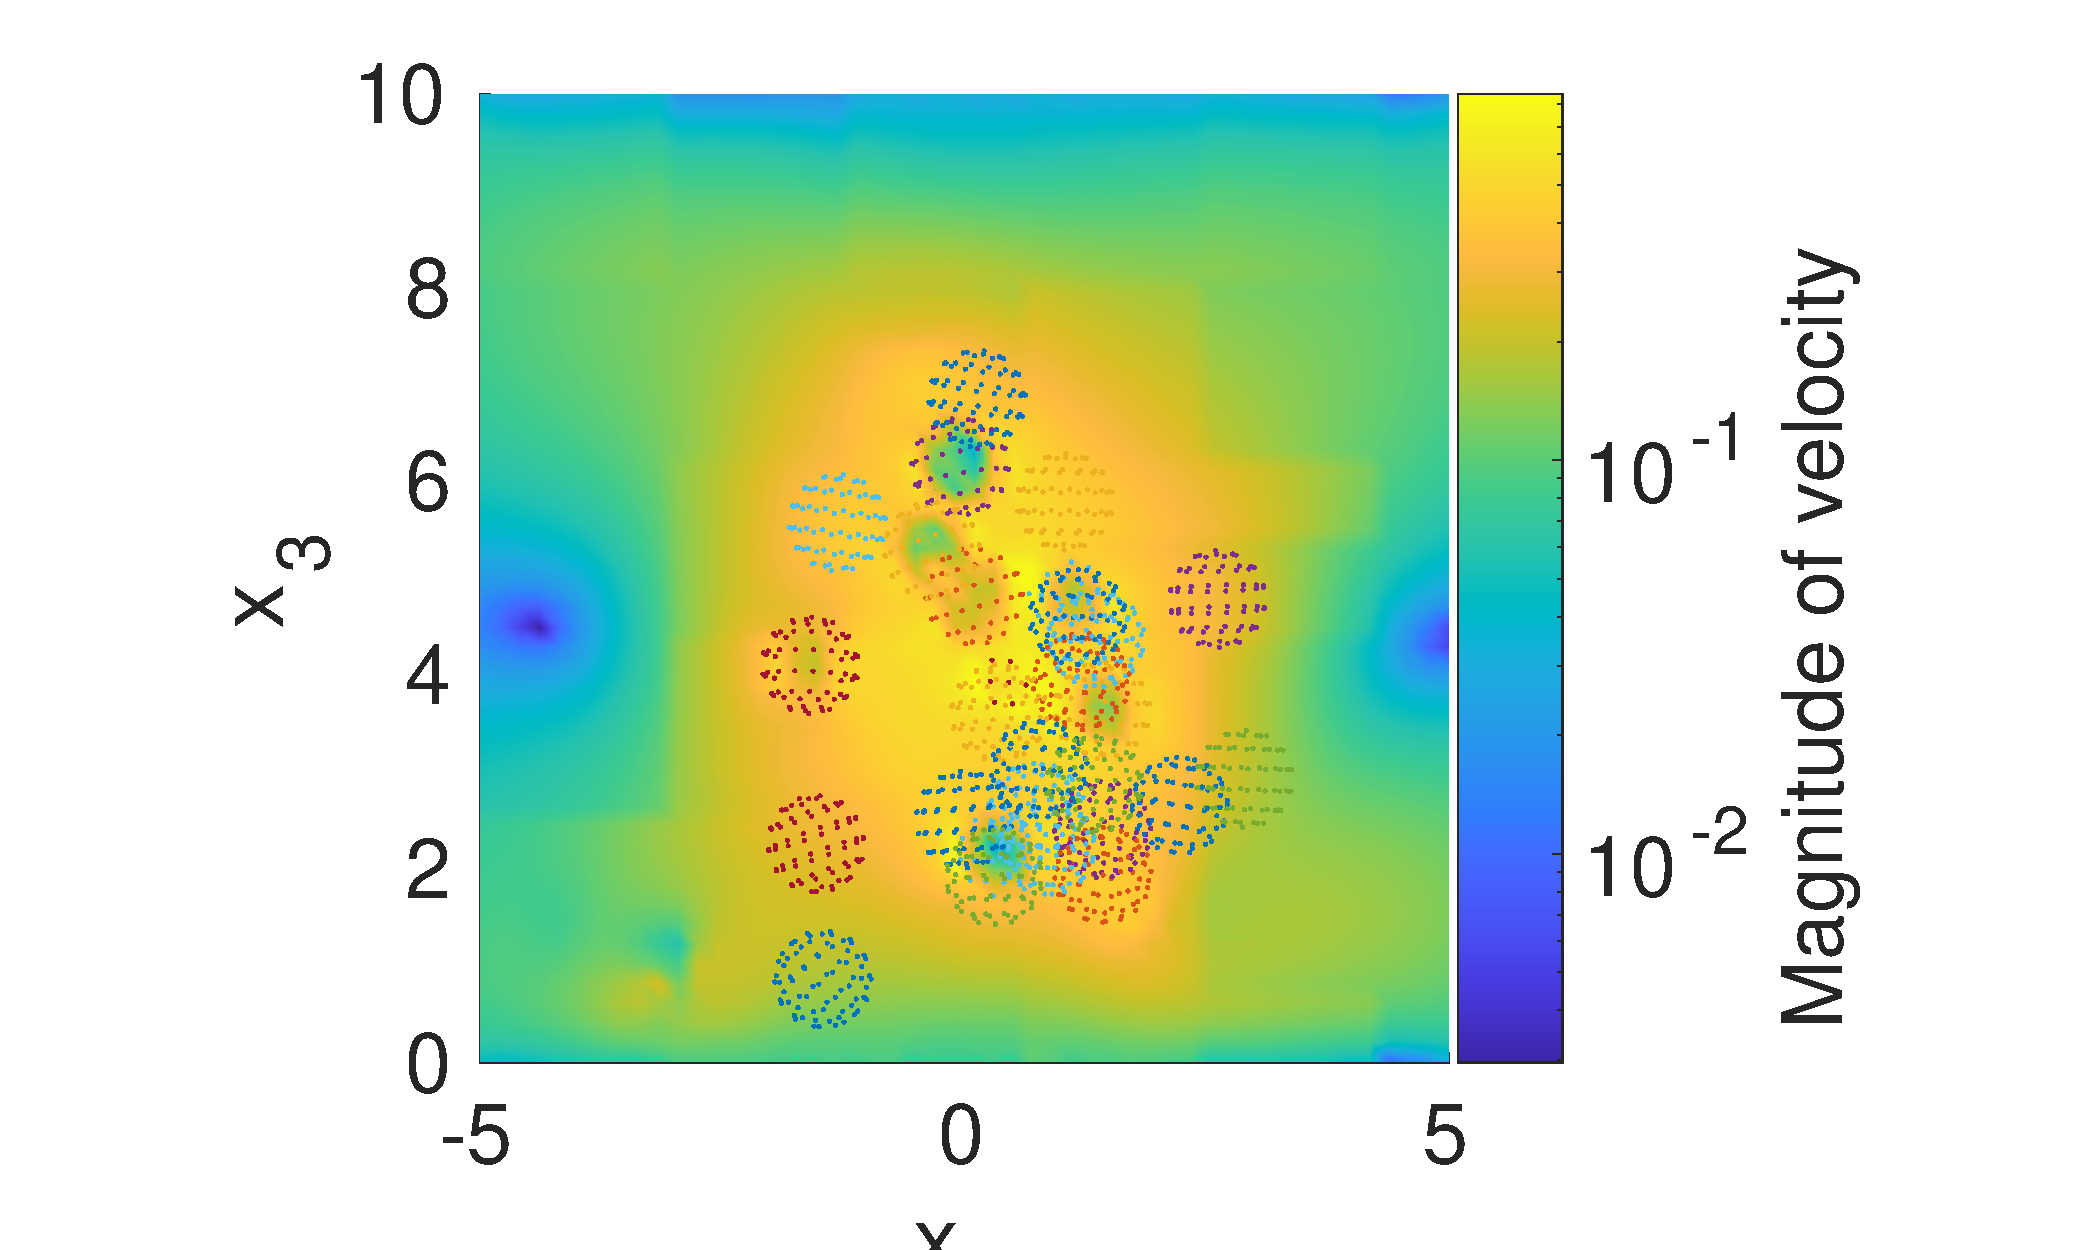
\includegraphics[width=\textwidth]{Images/squirmers/Gyro-3.pdf}
    \caption[]{\label{fig:squirmerC}}
\end{subfigure}
\begin{subfigure}[b]{0.22\textwidth}
    \centering
    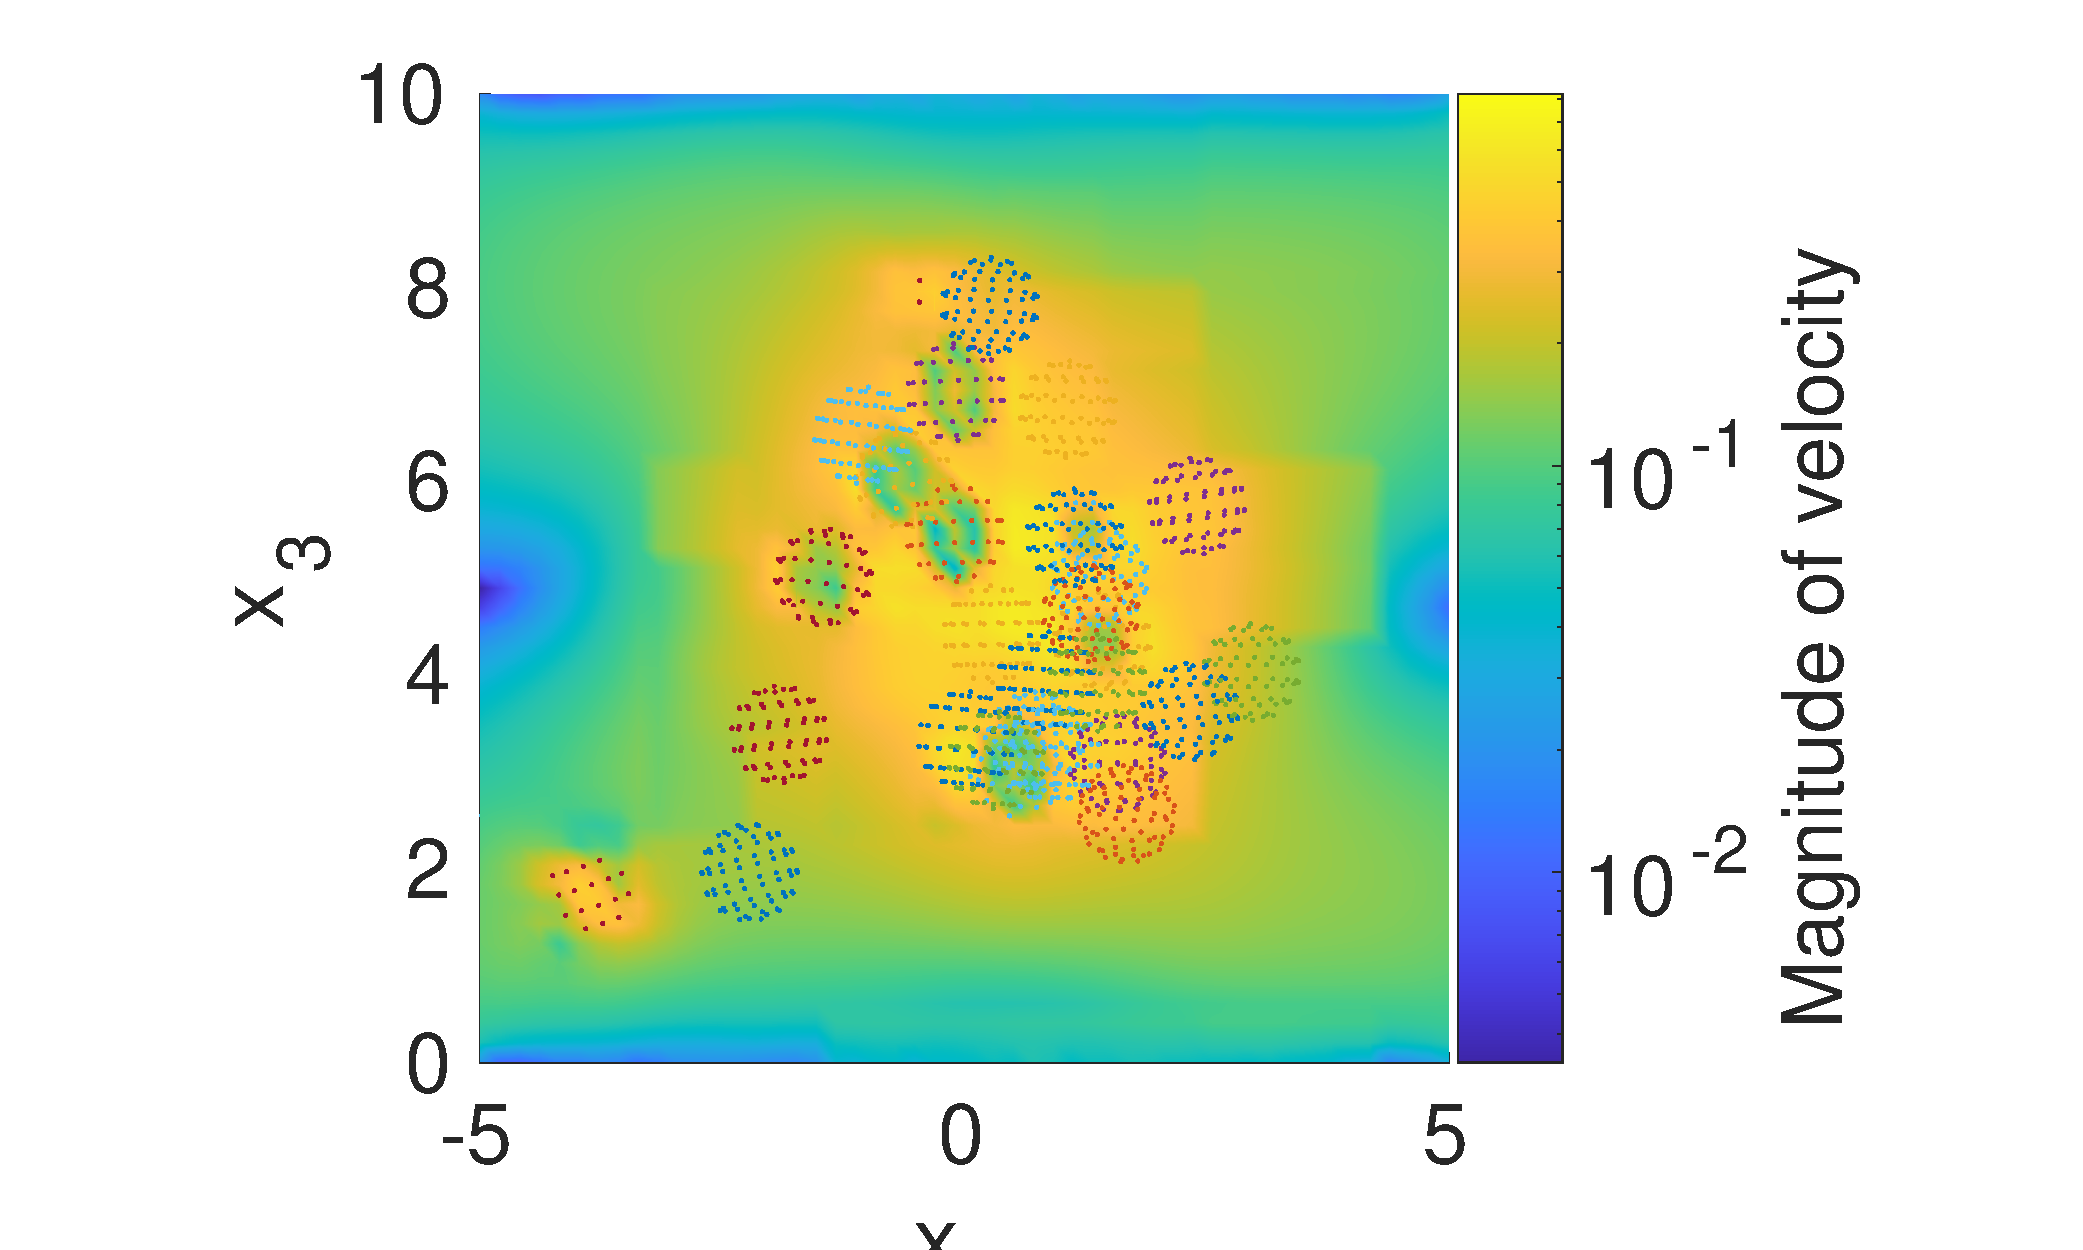
\includegraphics[width=\textwidth]{Images/squirmers/Gyro-4.pdf}
    \caption[]{\label{fig:squirmerD}}
\end{subfigure}
\vskip\baselineskip
\begin{subfigure}[b]{0.22\textwidth}
    \centering
    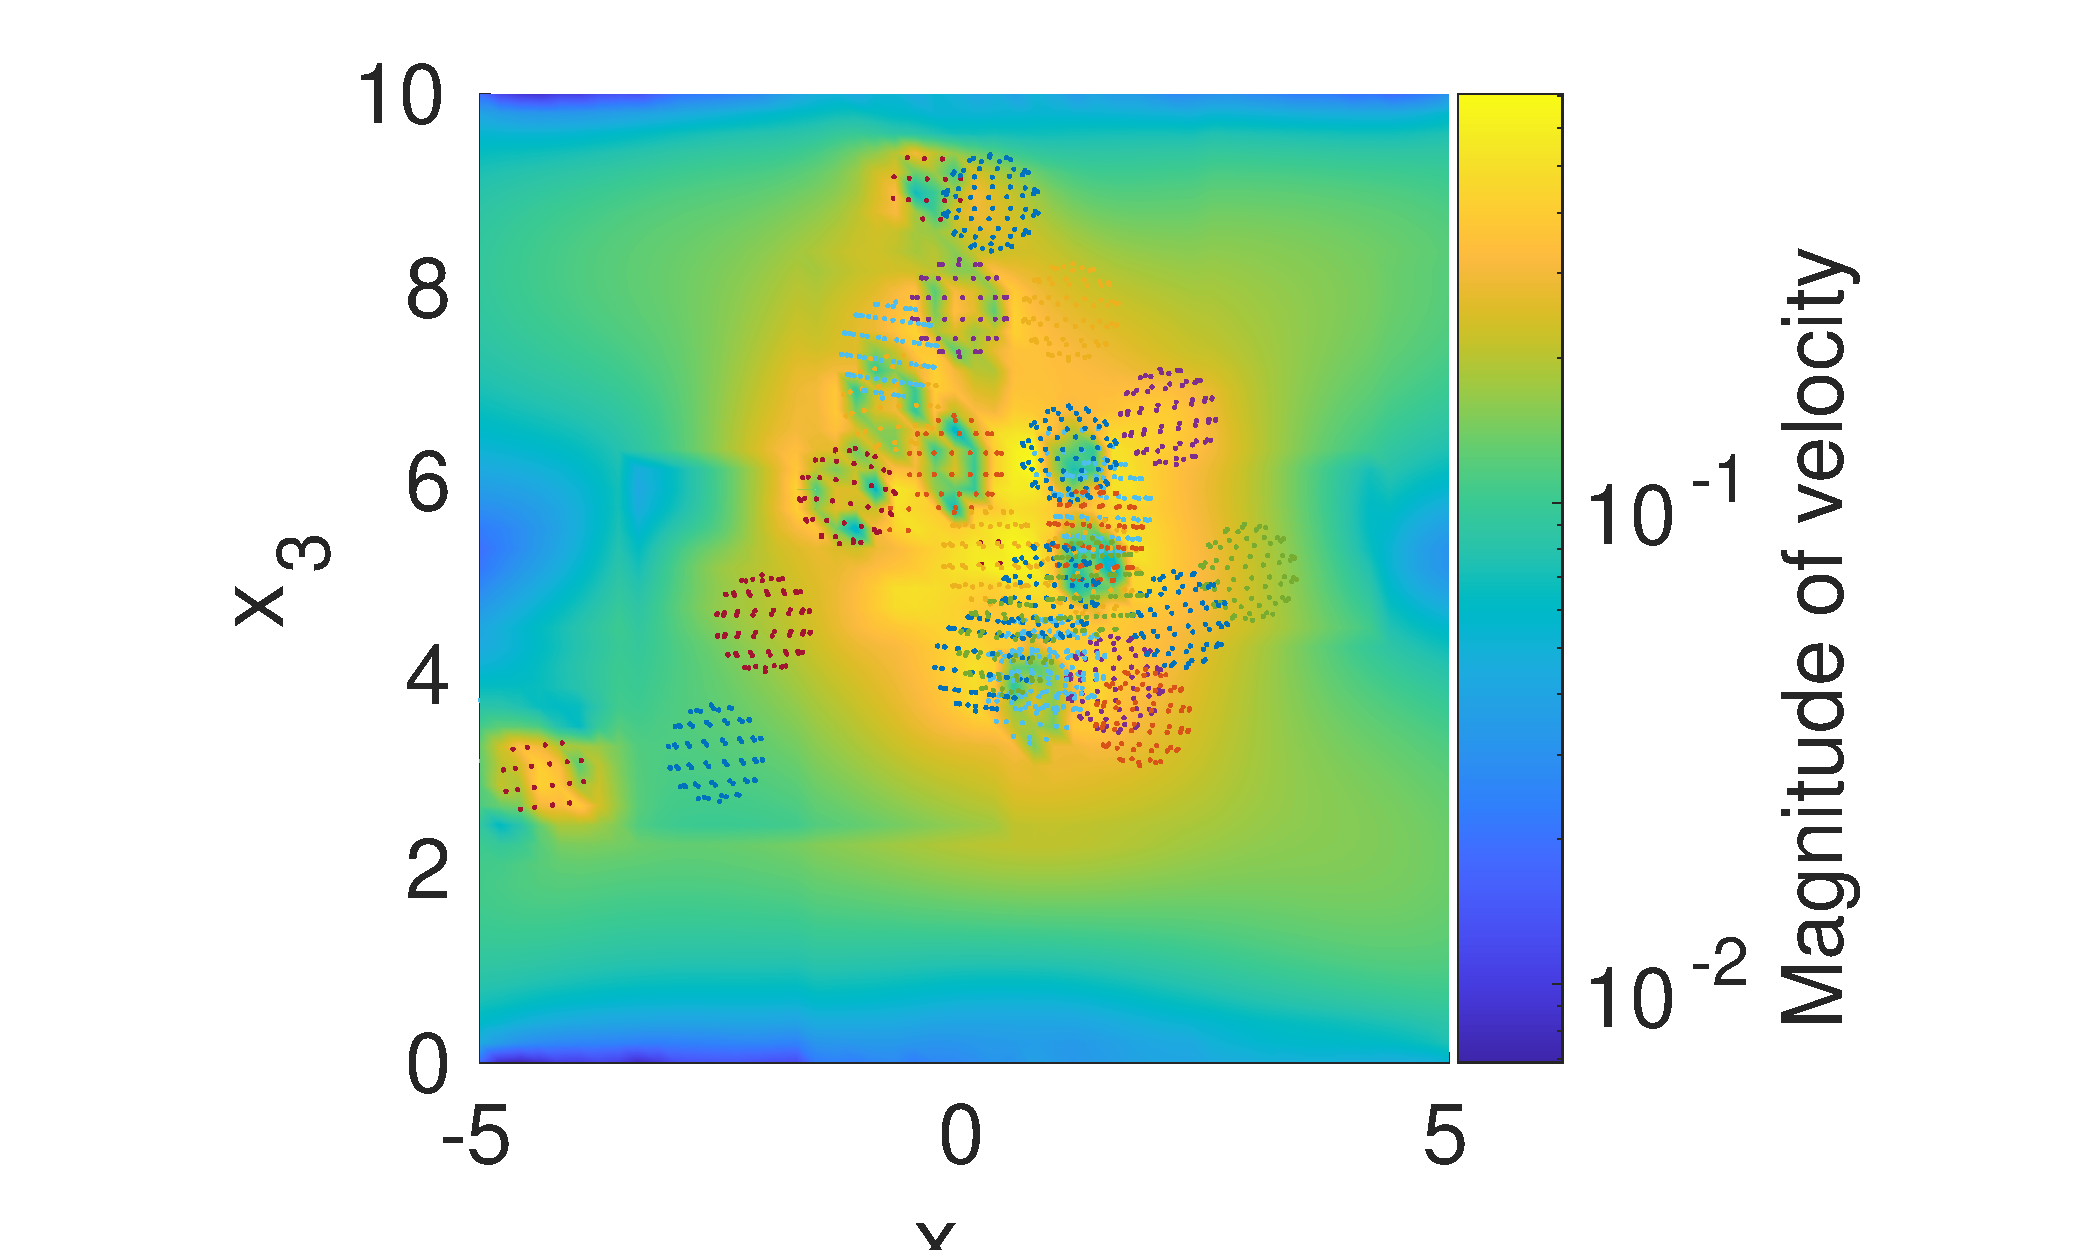
\includegraphics[width=\textwidth]{Images/squirmers/Gyro-5.pdf}
    \caption[]{\label{fig:squirmerE}}
\end{subfigure}
\begin{subfigure}[b]{0.22\textwidth}
    \centering
    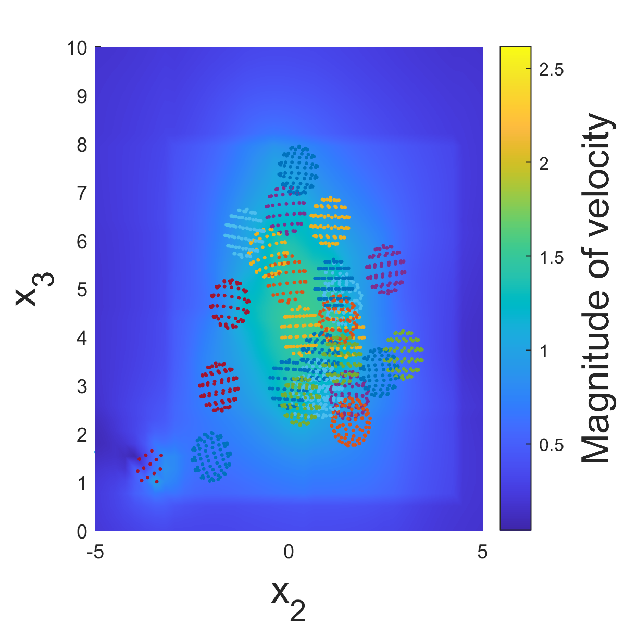
\includegraphics[width=\textwidth]{Images/squirmers/Gyro-6.pdf}
    \caption[]{\label{fig:squirmerF}}
\end{subfigure}
\begin{subfigure}[b]{0.22\textwidth}
    \centering
    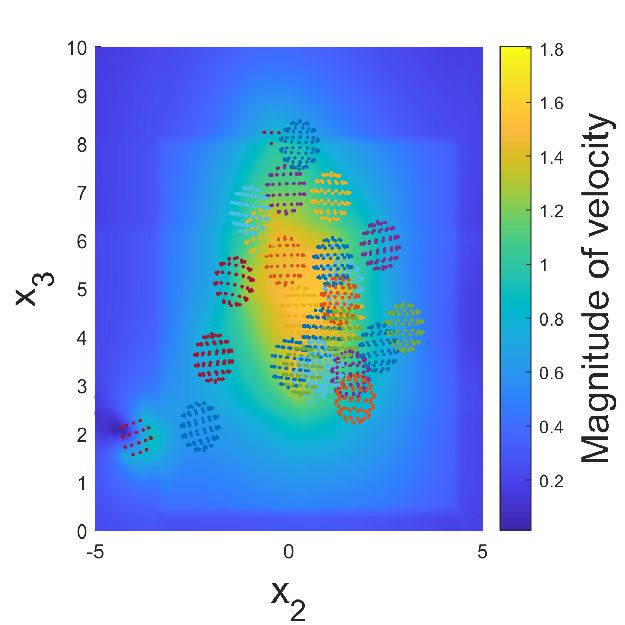
\includegraphics[width=\textwidth]{Images/squirmers/Gyro-7.pdf}
    \caption[]{\label{fig:squirmerG}}
\end{subfigure}
\begin{subfigure}[b]{0.22\textwidth}
    \centering
    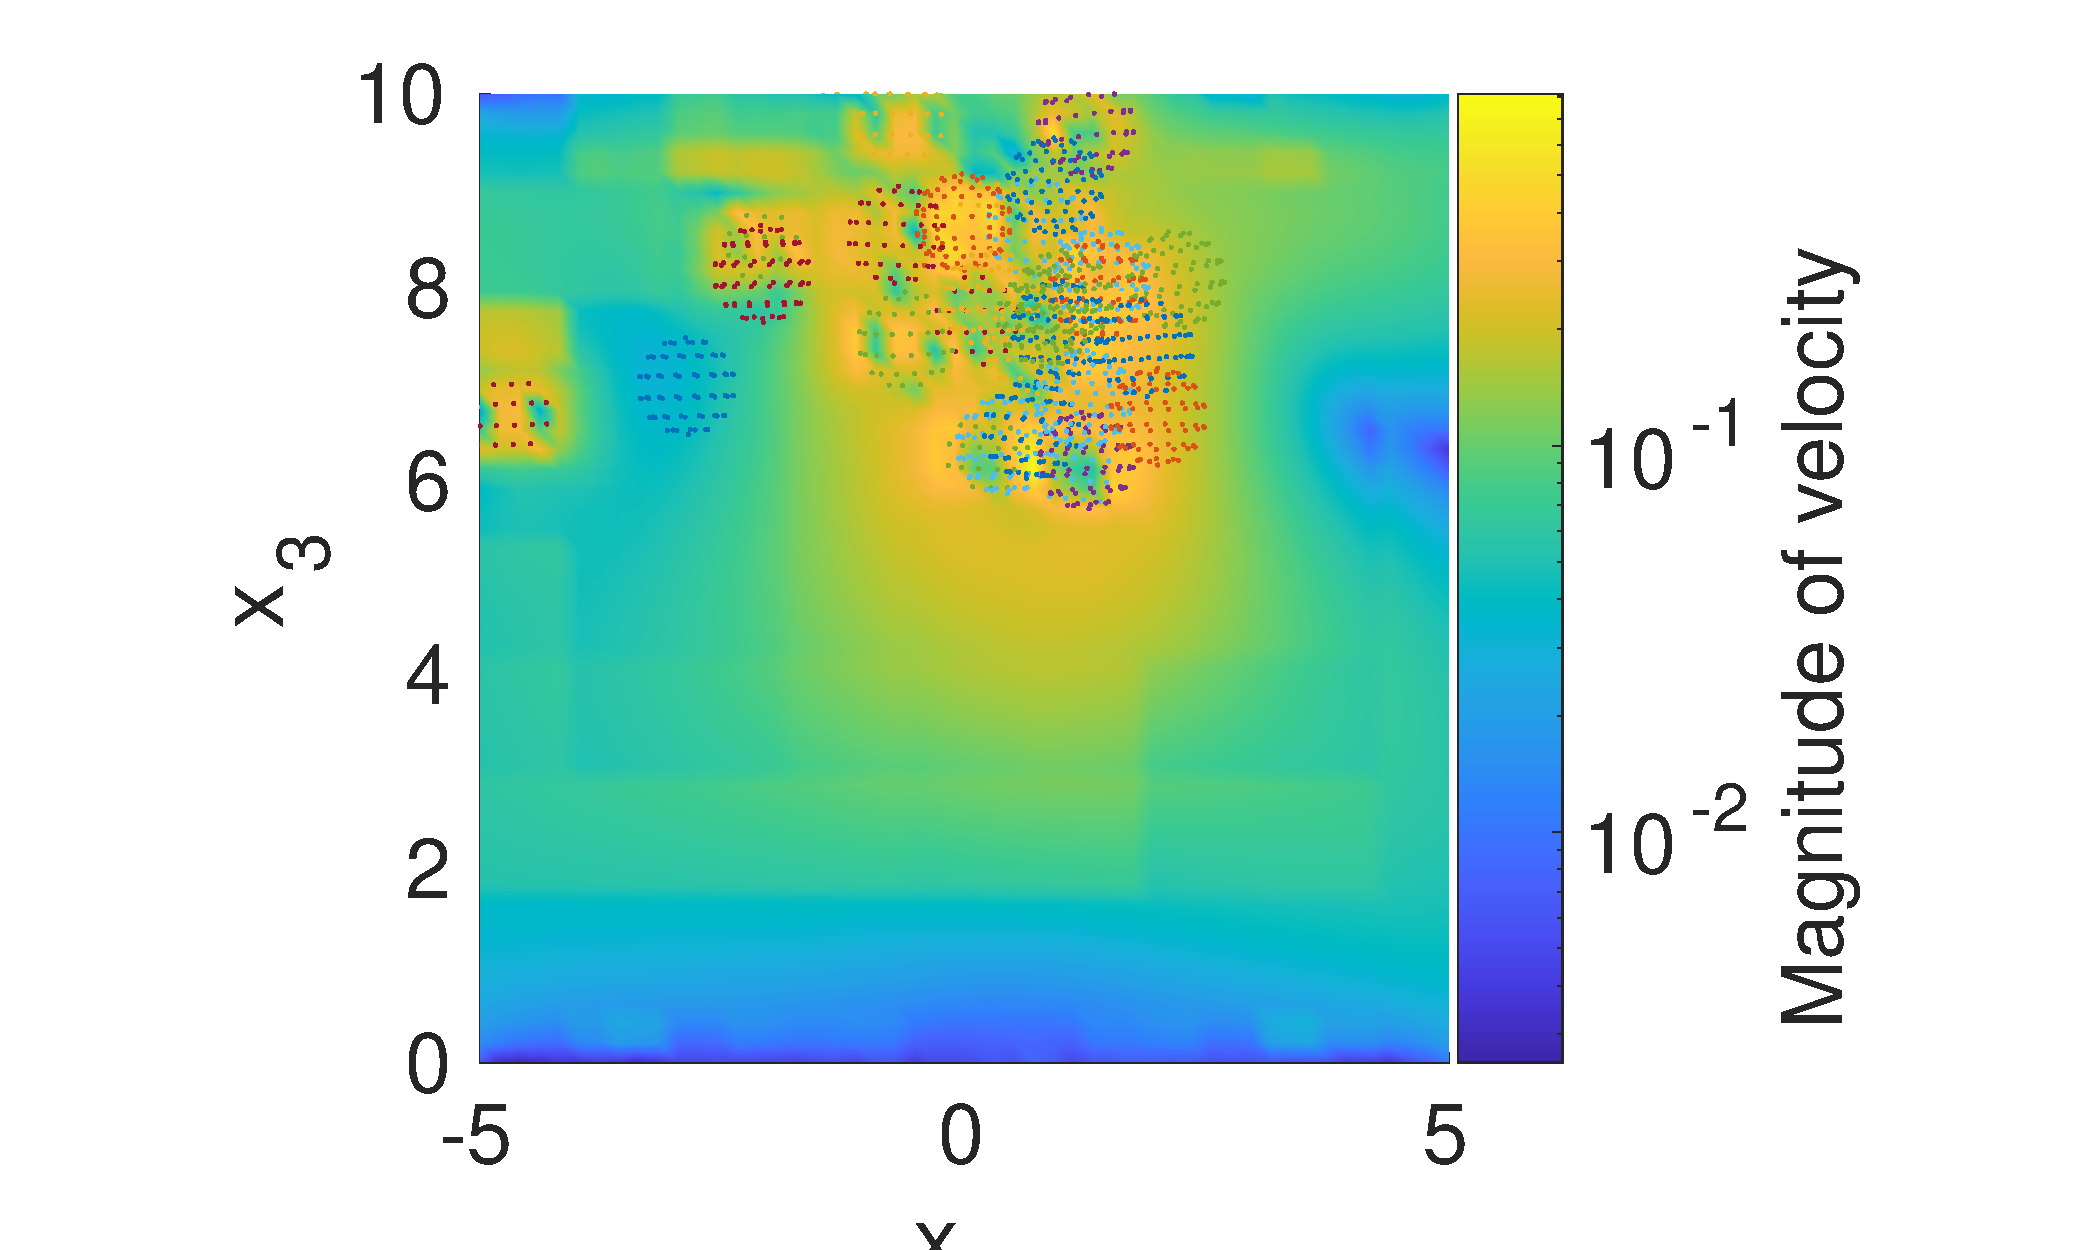
\includegraphics[width=\textwidth]{Images/squirmers/Gyro-8.pdf}
    \caption[]{\label{fig:squirmerH}}
\end{subfigure}
\label{fig:SquiremerGyro}
\caption[Position and velocity profile at 8 time steps of 50 squiremers randomly distributed at t=0.]{Position and velocity profile slice at $x_1=0$ are shown at 8 time steps of 50 squirmers randomly distributed at t=0. Two plates define the top and bottom of the simulations at $x_3 = 0$ and  $x_3 = 10$. (i-viii) show squirmer positions at t = 0, 0.74, 1.48, 2.212, 2.96, 3.70, 4.44 and 5.18 respectively.}
\end{figure}
